% mnras_template.tex   LaTeX template for creating an MNRAS paper

% Copyright (C) Royal Astronomical Society 2015
% Authors: Keith T. Smith (Royal Astronomical Society)


%%%%%%%%%%%%%%%%%%%%%%%%%%%%%%%%%%%%%%%%%%
%   PAQUETES INICIALES
%%%%%%%%%%%%%%%%%%%%%%%%%%%%%%%%%%%%%%%%%%

\documentclass[a4paper,fleqn,usenatbib]{mnras}     %a4paper=tamaño, fleqn=márgen ecuaciones, usenatbib=bibliografia
%\documentclass[a4paper,referee,fleqn,usenatbib]{mnras}                   


% MNRAS is set in Times font. If you don't have this installed (most LaTeX installations will be fine) or prefer the old Computer Modern fonts, comment out the following line
%\usepackage{newtxtext,newtxmath} 						% OJO: NO ME FUNCIONABA Y LA COMENTÉ. DESCOMENTÉ LÍNEAS 16 Y 17
% Depending on your LaTeX fonts installation, you might get better results with one of these:
\usepackage{mathptmx}    % OJO: VENIA COMENTADA
\usepackage{txfonts}         % OJO: VENIA COMENTADA
\usepackage[T1]{fontenc}
\usepackage{ae,aecompl}
\usepackage{graphicx}	% Including figure files
\usepackage{amsmath}	% Advanced maths commands
\usepackage{amssymb}	% Extra maths symbols
\usepackage{longtable}   %table

% Please keep new commands to a minimum, and use \newcommand not \def to avoid overwriting existing commands. Example:
%\newcommand{\pcm}{\,cm$^{-2}$}	% per cm-squared
%Incluidos por mi:
\newcommand{\Ha} {H$\alpha$}      		% Halpha
\newcommand{\Hb} {H$\beta$}      		% Hbeta
\newcommand{\NII} {[\ion{N}{ii}]}            % [NII]
\newcommand{\SII} {[\ion{S}{ii}]}             % [SII]
\newcommand{\OIII} {[\ion{O}{iii}]}          % [OIII]
\newcommand{\A} {\AA{}}                  	% amstrong
\newcommand{\kms}{\,km\,s$^{-1}$}	       % km/s
\newcommand{\Ne}{n$\mathrm{_e}$}	       % densidad electronica ne
\newcommand{\Te}{T$\mathrm{_e}$}	       % temperatura electronica Te



% Title of the paper, and the short title which is used in the headers.
\title[The wild west of the Orion nebula]{The wild west of the Orion nebula}


% The list of authors, and the short list which is used in the headers.
% If you need two or more lines of authors, add an extra line using \newauthor
\author[Fern\'andez-Mart\'in et al.]{                                            % short list which is used in the headers
Alba Fern\'andez-Mart\'in ,$^{1}$\thanks{E-mail: a.fernandez@crya.unam.mx}            % authors
William J. Henney,$^{1}$
M. Teresa Garc\'ia-D\'iaz$^{2}$
\newauthor                                                       % si ocupan mas de una linea ponerlo tras esto
and S. Jane Arthur$^{1}$
\\                                      %MUY IMPORTANTE: NO PONER ESPACIO DESPUÉS DE ESTO QUE SE LÌA
% List of institutions
$^{1}$Instituto de Radioastronom\'ia y Astrof\'isica, UNAM, Apartado Postal 3-72, 58090 Morelia, Michoac\'an, M\'exico\\
$^{2}$Instituto de Astronom\'ia, UNAM, Km 103 Carretera Tijuana-Ensenada, 22860 Ensenada, Baja California, M\'exico\\
%$^{3}$Institution3
}


% These dates will be filled out by the publisher
\date{Accepted XXX. Received YYY; in original form ZZZ}

% Enter the current year, for the copyright statements etc.
\pubyear{2016}

% Don't change these lines
\begin{document}
\label{firstpage}
\pagerange{\pageref{firstpage}--\pageref{lastpage}}
\maketitle



%%%%%%%%%%%%%%%%%%%%%%%%%%%%%%%%%%%%%%%%%%
%   ABSTRACT AND KEYWORDS
%%%%%%%%%%%%%%%%%%%%%%%%%%%%%%%%%%%%%%%%%%

% Abstract of the paper
\begin{abstract}
      %Single paragraph,not more than 250 words and no references.\\
      %Aims.\\
      %Methods.\\
      %Results.\\
\end{abstract}

% Select between one and six entries from the list of approved keywords.
\begin{keywords}
keyword1 -- keyword2 -- keyword3 -- keyword4 -- keyword5 -- keyword6
\end{keywords}





%%%%%%%%%%%%%%%%%%%%%%%%%%%%%%%%%%%%%%%%%%
%   1. INTRODUCCION
%%%%%%%%%%%%%%%%%%%%%%%%%%%%%%%%%%%%%%%%%%
\section{Introduction}\label{sec:introduction}


%Describir LL1, LL2 y LL3, si no poner sus referencias en la seccion \ref{sec:red_large_structures}.






%%%%%%%%%%%%%%%%%%%%%%%%%%%%%%%%%%%%%%%%%%
%   2. OBSERVACIONES Y REDUCCION
%%%%%%%%%%%%%%%%%%%%%%%%%%%%%%%%%%%%%%%%%%


\section{Observations and data reduction}\label{sec:obs_and_red}



%---------------------------------
%   2.1 OBSERVACIONES
%---------------------------------
\subsection{Observations}\label{sec:observations}
High-resolution spectroscopic observations were obtained at the 2.1-m telescope of the Observatorio Astron\'omico 
Nacional San Pedro M\'artir (Baja California, M\'exico) in a f/7.5 configuration using the MES-SPM instrument (Manchester Echelle 
Spectrometer; \citealt{Meaburn2003}). A total of 62 spectra were obtained from seven sets of observations carried 
out in 2006, 2007, 2010, 2013 and 2015. The number of positions acquired in each set of observations, dates, exposition 
times and airmass during the observations are summarized in Table \ref{table:logSPM}.


For the 2006, 2007a, 2007b and 2010 observations the instrument was equipped with the detector SITE-3 CCD, which is an array 
of 1024$\times$1024 (24$\mu$m) pixels giving a spatial resolution of 0.321 arcsec/pix (without considering the binning). On the 
other hand, the CDD used for the 2013a, 2013b and 2015 sets, Marconi-2, is a detector with 2048$\times$2048 square pixel, each 13.5 $\mu$m, 
giving a spatial resolution of 0.176 arcsec/pix (without considering the binning). The slit width was set at 150$\mu$ (1.95 arcsec 
on the sky) throughout the observation and it was oriented in the north-south direction for 2006, 2007a, 2007b and 2010 observations and in the east-west 
direction for the 2013a, 2013b and 2015 ones.  

In order to establish the exact position of the slit in each pointing we took direct slit images of short duration, in which the diffraction 
grating was replaced by a mirror. Additionally, thorium-argon lamp spectra were taken for wavelength calibration between each slit position.

Finally, taking the seven data sets into account, we get 56 slit-positions in \Ha, \NII$\lambda$6548 and \NII$\lambda$6584, lines spanning an interval 
of 217~arcmin in RA and 9~arcmin in DEC. In addition, exposures in \SII$\lambda$6717 and \SII$\lambda$6730 were also observed in four 
pointings and \OIII$\lambda$5007 in two positions, as indicated in Table \ref{table:logSPM}. In order to illustrate the spatial distribution of the 
observations in Fig. \ref{fig:slits_distribution} we show the 56 slit positions observed in \Ha+\NII~plotted over an \Ha~image obtained from \citet{DaRio2009}.\\



%-------------------------------------------TABLA: OBSERVACIONES---------------------------------------------------------------------------------------------------------
\begin{table*}
\caption{Summary of the data set observed with the spectrograph MES-SPM.} 
\label{table:logSPM} 
\centering 
\begin{tabular}{l c c c c c c c }
\hline

Set name  &           Dates     & \# Slits$^{[a]}$  & Orientation   & Spatial resolution$^{[b]}$ &  Cover area       & Exp. time$^{[c]}$ &  Airmass$^{[d]}$ \\
          &                     &                   &               &    (arcsec\,pix$^{-1}$)    & (arcmin$^{2}$)    &      (s)          &                  \\
\hline
2006      &  2006 Feb 5         &    11/0/0         &  north-south   &              0.624         &  6$\times$6       & 300(3)/600(8)     &      1.68        \\
2007a     &  2007 Jan 10        &    3/1/1          &  north-south   &              0.624         &  2$\times$6       &       600         &      1.67        \\
2007b     &  2007 Jan 13        &    7/0/0          &  north-south   &              0.624         &  14$\times$6      &       600         &      1.30        \\
2010      &  2010 Jan 15,16,17  &    17/3/1         &  north-south   &              0.624         &  17$\times$6      &  450(1)/600(20)   &      1.37        \\
2013a     &  2013 Feb 16,18,19  &    11/0/0         &  east-west   &              0.527         &  100$\times$2     &  450(1)/600(10)   &      1.52        \\            
2013b     &  2013 Dec 11        &    5/0/0          &  east-west   &              0.527         &  114$\times$0.2   &          600      &      1.49        \\
2015      &  2015 Feb 3         &    2/0/0          &  east-west   &              0.351         &  88$\times$0.2    &          600      &      1.29        \\
\hline
\end{tabular}
\begin{list}{}{}\footnotesize{
\item $^{[a]}$ Number of slit positions observed in \Ha+\NII$\lambda\lambda$6548,6584 / \SII$\lambda\lambda$6717,6731 /  \OIII$\lambda$5007.
\item $^{[b]}$ Final spatial resolution taking the spatial binning into account.
\item $^{[c]}$ 2006, 2010 and 2013a spectra were taken with different exposition times (separated by a bar). Number of position acquired with each exposition 
time are indicated in brackets. This was taking into account when combining images in the data reduction.
\item $^{[d]}$ Mean value during the observations.
}
\end{list}
\end{table*}
%----------------------------------------------------------------------------------------------------------------------------------------------------


\begin{figure*}
	    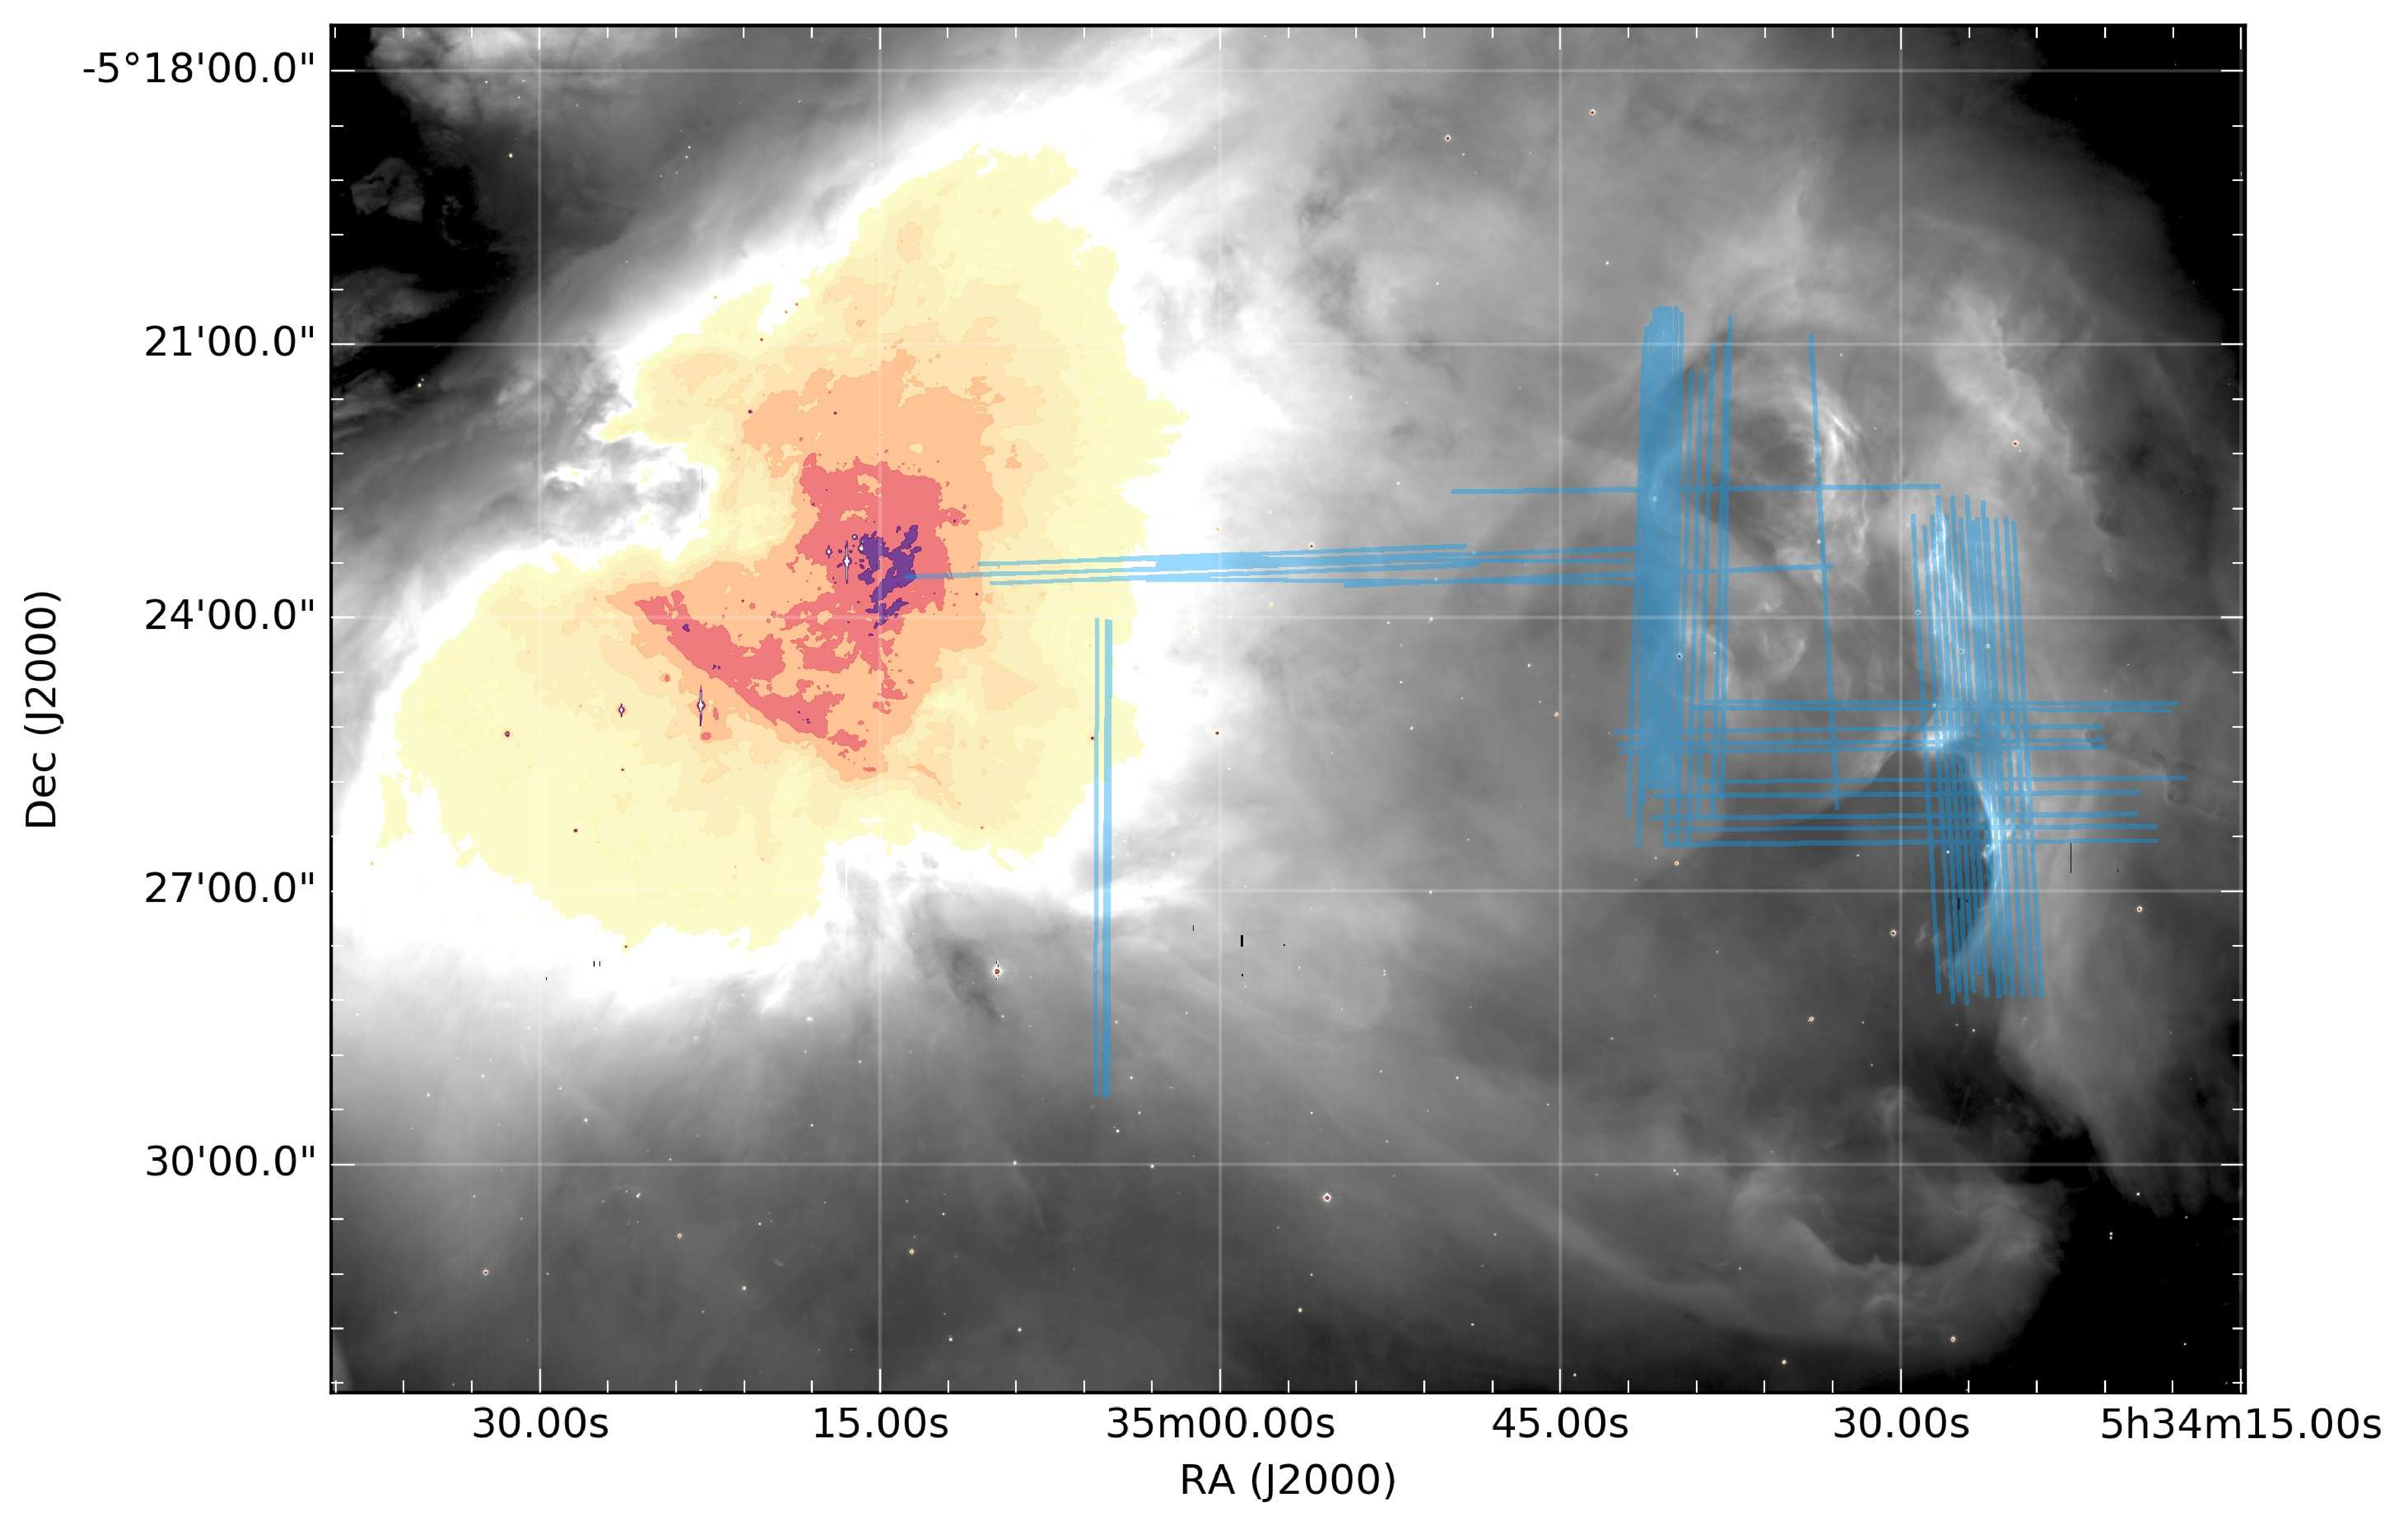
\includegraphics[width=\textwidth]{Figs/fov_with_slits.pdf}
	    \caption{Positions and orientations of the spectroscopic settings observed in \Ha+\NII~with MES-SPM (in blue) plotted over 
                 the \Ha~image of the western region of the Orion nebula obtained from \citet{DaRio2009}. North is up and east to the left.}
    \label{fig:slits_distribution}  
\end{figure*}





%---------------------------------
%   2.2 REDUCCION DATOS
%---------------------------------
\subsection{Data reduction}\label{sec:reduction}
The spectra were reduced using {\small IRAF}\footnote{The Image Reduction and Analysis Facility IRAF is 
distributed by the National Optical Astronomy Observatories, which are operated by Association of Universities 
for Research in Astronomy, Inc., under cooperative agreement with the National Science Foundation.} by 
following the standard procedure for 2D spectroscopic observations (bias subtraction, flat-fielding and cosmic 
ray removal). The wavelength calibration was performed using thorium-argon arcs taken between each slit position. 


After transforming all the spectra to a common heliocentric velocity frame, we performed a series of further 
corrections to obtained well calibrated spectra in a self-consistent way.
\begin{enumerate}

\item An astrometric solution was found for each of the spectra using nearby stars. This allowed us to 
accurately determine the slit position of each exposure.

\item In order to compensate the variations in the sky transparency and seeing between exposures we compare 
our spectra with a deep \Ha~image of the region obtained from \citet{DaRio2009} with the Wide Field Imager (WFI) 
at the 2.2-m MPG/ESO telescope at La Silla. This was done by fitting a low-order Chebyshev polynomial to the 
spectra to WFI profile ratio. With this we obtained a brightness normalization factor for each spectra, as well as a 
correction for flux gradients along the slits. The corrections are typically lower than 15 percent. This comparison also allowed 
us to flux-calibrate our spectra, using the spectrophotometry provided by \citet{Weilbacher2015} with MUSE in common regions. 
%Figure \ref{fig:flux_calibration} shows a three-panel plot with the flux calibration for one of the positions.

\item Continuum emission was removed by fitting a two-dimensional Chebyshev function. For each exposure a 
background section was selected including only line-free regions of the spectrum (we use an excluded velocity window 
of -10 to +40 \kms in heliocentric velocity around the line core). In addition we use an intensity threshold to distinguish high-velocity 
knots from noise.
\end{enumerate}

Figure \ref{fig:calibrated_spectra} shows the resultant calibrated two-dimensional spectra in \Ha~(top row) and \NII~(bottom row) for three 
representative slit positions.


\begin{figure}
    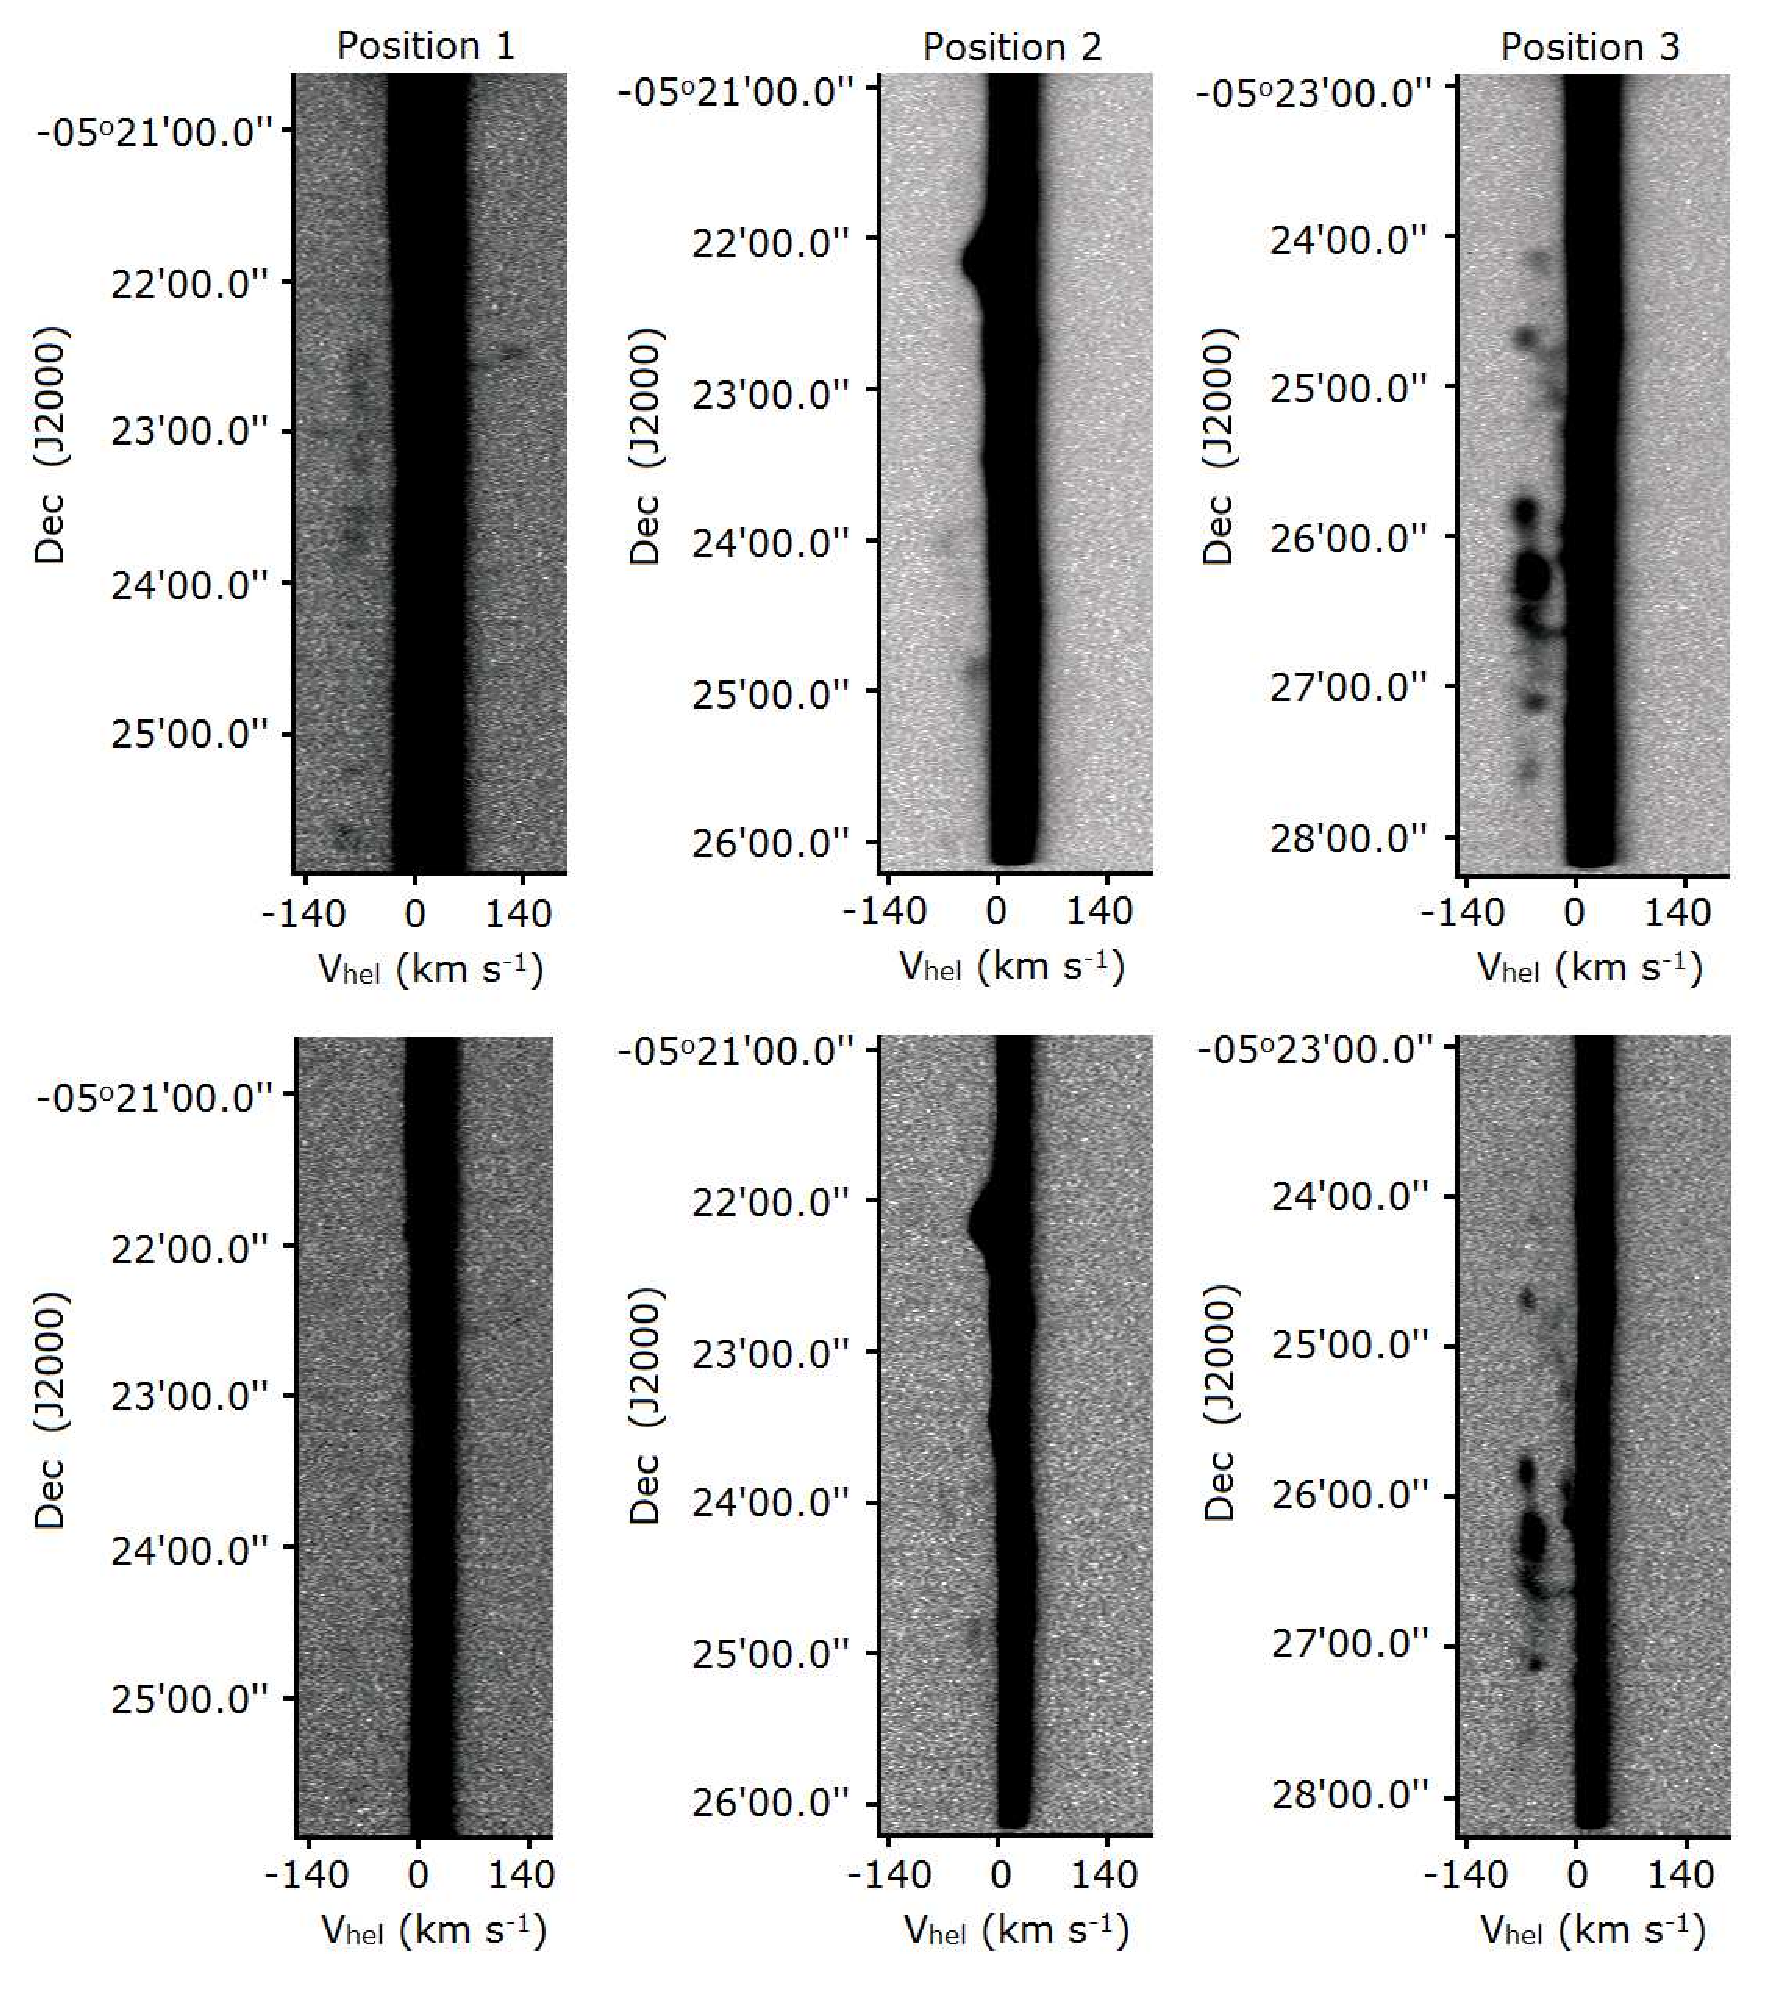
\includegraphics[width=\columnwidth]{Figs/calibrated_spectra.pdf}
    \caption{Calibrated two-dimensional spectra for three representative slit positions. The top row shows the \Ha~emission line and 
      the bottom one the \NII$\lambda$6584~emission line.}
    \label{fig:calibrated_spectra}
\end{figure}











%%%%%%%%%%%%%%%%%%%%%%%%%%%%%%%%%%%%%%%%%%
%   3. MAPAS DE ISOVELOCIDADES
%%%%%%%%%%%%%%%%%%%%%%%%%%%%%%%%%%%%%%%%%%
   
\section{Isovelocity maps}\label{sec:maps}

\begin{figure*}
		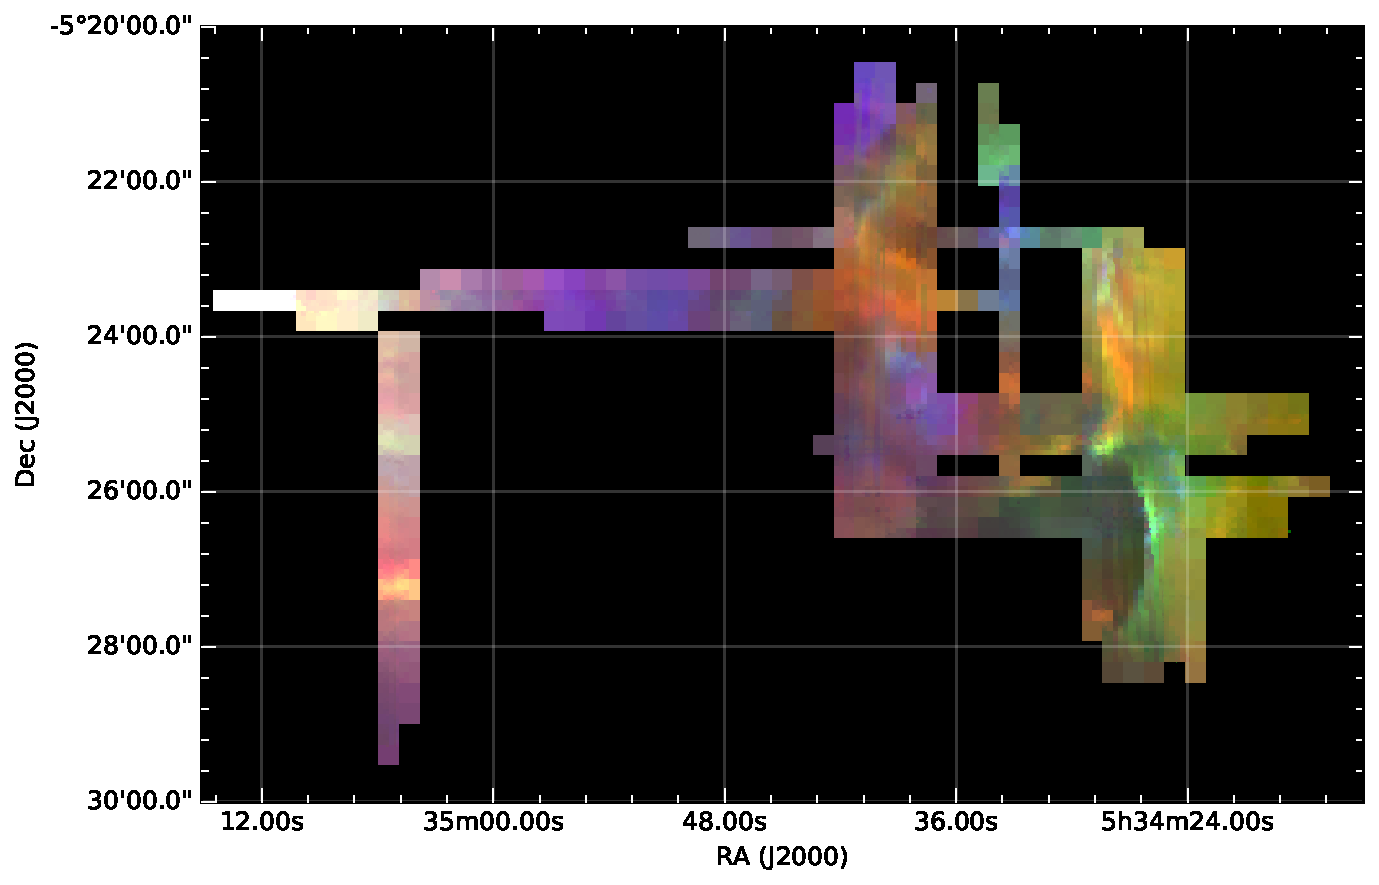
\includegraphics[width=\textwidth]{Figs/rgb_core_NII.pdf} 
		\caption{RGB composite image of the western region of the Orion nebula obtained from the \NII~isovelocity  maps. Red corresponds
		to the channel maps with heliocentric velocity between +30 and +50~\kms, green between +10 and +30~\kms and blue between 
		-10 and +10~\kms. North is up and east to the left.}
    \label{fig:isov_maps}
\end{figure*}

In order to better reveal the spatio-kinematical patterns in the observed region, the slit spectra were combined and interpolated 
to produce isovelocity channel maps. To that end, we carried out the following steps.

First, we built an orthogonal RA-DEC grid placing all the slits onto there by looping over slit profiles extracted in a 
given wavelength (helocentric velocity) window. On those grid pixels in which two or more slits fall, the intensity was estimated 
as the mean weighted by the slit quality. Grid pixels where no slit falls were left transparent.

Due to observational The results shown in the previous section provide the velocity of the bow-shocks in our line of sight. However, to draw a tridimensional picture of the shock it is necessary to determine their velocity in the plane of the sky, i.e. to measure the proper motions.

With this aim a rough estimation of the proper motions of the large scale identified in our region was performed. We resorted to images of the western region of the Orion nebula observed with the ACS instrument of the HST which observations are separated almost 10 years. The first-epoch image was taken on April 26th 2005 while the second image was observed on March 2th 2015. The data used are calibrated and have a relative astrometric correction performed, however, to measure accurate displacements in the features we carry out an absolute astrometric calibration between both images.

We blink our matches images looking for nebular motions. In three of the five red bow shocks studied (NE, SW-S and SW-W).we find spatial displacement between the two epochs observed. In addition, we also detect clear motions in a little arc close to the SW-W red bow sock (identified as SW-W arc). For measurement, the profiles of the shocks were traced and compared in a manual mode. The displacements of the profiles between the two epochs were then measured. Taking into account that the time passed from the first epoch to the second is 3957 days (3.10782$\times$10$^8$ seconds), we derived the velocity of each shock in the plane of the sky. Results are shown in Table \ref{table:propermotions}.differences between each set of observations (i.e. spatial resolution and seeing) we generated 
multi-resolution maps in order to not degrade the quality of the better spectra. To do that, we build several isovelocity 
maps onto grids with binning of 2 (better resolution), 4, 8, 16 and 32 (worst resolution).

Finally, all the grids were combined to obtain multigrid smoothed channel maps with a spatial resolution ranging 
from 0.5 to 15.1 arcsec\,pix$^{-1}$. We created maps in several velocity ranges to find kinematical structures at different 
velocities: the narrow band channels cover velocities from -10 to -110 \kms and from +10 to +170 \kms~in steps of 
20 \kms, while the wide bands span from +0 to +60, -60 to +0 and -120 to -60 \kms. The line core is also sampled in the 
channel ranging from -10 to +10 \kms. These isovelocity maps were performed only in \Ha~and \NII~emission lines, because 
in \SII~and \OIII~the spatial coverage of the observations is too small.\\


A particularly useful method of identifying large-scale velocity systems is to study images that are color-coded to simultaneously 
show different velocity ranges. In Fig. \ref{fig:isov_maps} we present combined isovelocity channel maps for \NII~ covering the 
heliocentric velocity range from -10 to +50 \kms. 

The analysis of the isovelocity channel maps reveal a rich harvest of results that can be subdivided into several distinct topics. 
In the following two sections we provide an empirical description of the kinematical features observed by using the isovelocity 
channel maps and the position-velocity spectra. First we describe major features seen in the western outskirts of the Orion 
nebula. Later we focus on blue and redshifted knots with high radial velocity. 

When naming new compact objects, we have followed the convention established by \citet{ODell1994} that evokes the two-dimensional 
position on the plane of the sky. The first four digits indicate the position of right ascension 
and the second three digits the position in declination (both in J2000 epoch and respect to 
$\alpha$=5${^h}$3X${^m}$:XX${^s}$.X $\delta$=-5$^{\rm o}$:2X$^{\rm '}$:XX$^{\rm ''}$).




%%%%%%%%%%%%%%%%%%%%%%%%%%%%%%%%%%%%%%%%%%%%%%%%%
%   4. ESTRUCTURAS GRANDES= RED BOW SHOCKS
%%%%%%%%%%%%%%%%%%%%%%%%%%%%%%%%%%%%%%%%%%%%%%%%%
\section{Large-scale structures}\label{sec:red_large_structures}

\begin{figure*}
   %\includegraphics[width=\textwidth]{Figs/rgb_red_Ha.pdf}  FIGURA POR HACERT
    \caption{\textbf{FIGURA POR HACER (WILL)}: Imagen WFI con estructuras a gran escala (red bow shocks) identificadas.}
    \label{fig:red_features}
\end{figure*}

The Western Wall is is a sharp step function in the nebula surface brightness, visible as the vertically oriented bright green
feature on the right hand side of Fig. \ref{fig:isov_maps}. The southern portion of the Wall is one of the most prominent 
large scale features visible in direct images of the outskirts of the Orion Nebula, extending roughly 2.5~arcmin in the N--S 
direction from 4276-751 to 4270-544, with a slight concavity that faces East towards the Trapezium. On the East side of the 
Wall is a region of low \Ha~surface brightness, which increases by a factor of 2--3 over a scale of \(\approx 10\)~arcsec at the 
position of the Wall to give a thick plateau that extends \(\sim 1\)~arcmin to the West.

At the North end of this portion of the Wall is a bright Ionized Clump of emission, centered on 4283-521 and with diameter 
of \(\approx10\)~arcsec.  There are indications that the Wall extends further North than this clump, but it becomes confused 
with other structures superimposed on it. \citet{ODell2015} classified it as a shock, but it does not appear to be moving.\\

At least four bow-shocks lie in the western part of our observation FoV. These features show velocities slightly redshifted with respect to 
the systematic velocity of the nebula and their appearance is detected in both \Ha~and \NII~isovelocity maps. The bow-shocks identified are 
illustrated in Fig. \ref{fig:red_features}. To describe their location we use their positions relative to the Wall. In addition, in order to 
confirm the identification and make precise locations of the structures we resort to high spatial resolution images obtained from \citet{DaRio2009} 
with the WFI (described above), \citet{Bally2006} with the Advanced Camera for Surveys (ACS) of the Hubble Space Telescope and \citet{Robberto2013} 
also with the ACS (hereinafter D09, B06 and R13, respectively). 


%NE 
The largest of the four bow-shocks is located on the northeast side of the Wall (we identified it as NE red-bow shock). It crosses LL2, but is 
oriented in its opposite direction, towards the west part of the nebula.  The channel maps reveal that it is moving with velocities from +0 
to +50 \kms~in both \Ha~and \NII, although some regions show velocities up to 90 \kms~in \Ha.  The morphology of this bow  is very 
well defined in the high-spatial resolution images from D09, B06 and R13, especially in B06 where it seems to be a region composed of 
various shocks moving toward the west. 

 %NW
The brighter, west-facing bow-shock we identify is located beyond the northwest of the Wall (called NW red bow-shock) and it seems to mimic the orientation of the 
northeast one. The bow-shock is well defined in \Ha, detected at velocities from +10 to +70 \kms, but is not clear in the \NII~maps, in 
which there are extended emission at the north of the bow-shock moving in the same range of velocities. Attending to the images, this region 
is spatially coincident only with the observations of D09 and R13, where it can be identified with the brighter 
emission of the bow-shock. However, this feature shows a less well defined bow shape than the others, as if only the edge of the parabolid 
were detected. This may be because it is located close to the boundary of the Wall, where the S/N is lower, preventing the detection the whole bow-shock.

%SW 
On the western side of the Wall we identified the third red bow-shock (called SW). The composite channel maps show that it is not so redshifted as the
other two presented above, moving with velocities from +10 to +50 \kms~in \Ha~and \NII. The bow-shock structure is clearly identifiable in 
the images obtained from D09 and R13 and it extends toward the southwest part of the Orion nebula. Analysing the \Ha~images we observed that in 
this bow-shock it can be distinguished two orientations: the first one moving to the west (SW-W) and the second one moving to the southwest 
(SW-S). To check this, the kinematical study of the SW shock will be performed differentiating the two possible sub-shocks.  

%SE  
Finally, the isovelocity maps reveal a red bow-shock located to the southeast that is dimmer than the other features described (identified as SE). It is 
detected in \Ha~and \NII~maps with velocities ranging from +10 to +50 \kms~and it crosses LL3. The structure of this bow-shock is not totally detected 
in the isovelocity maps because the slit positions observed do not spread enough in the southern part. Nonetheless, the whole bow morphology is 
perfectly identified in the \Ha~images from D09, B06 and R13.\\









%-----------------------------------
%   4.1 CINEMATICA RED BOW SHOCKS
%-----------------------------------
\subsection{Kinematics of the red bow shocks}\label{sec:shocks_kin}

\begin{figure}
    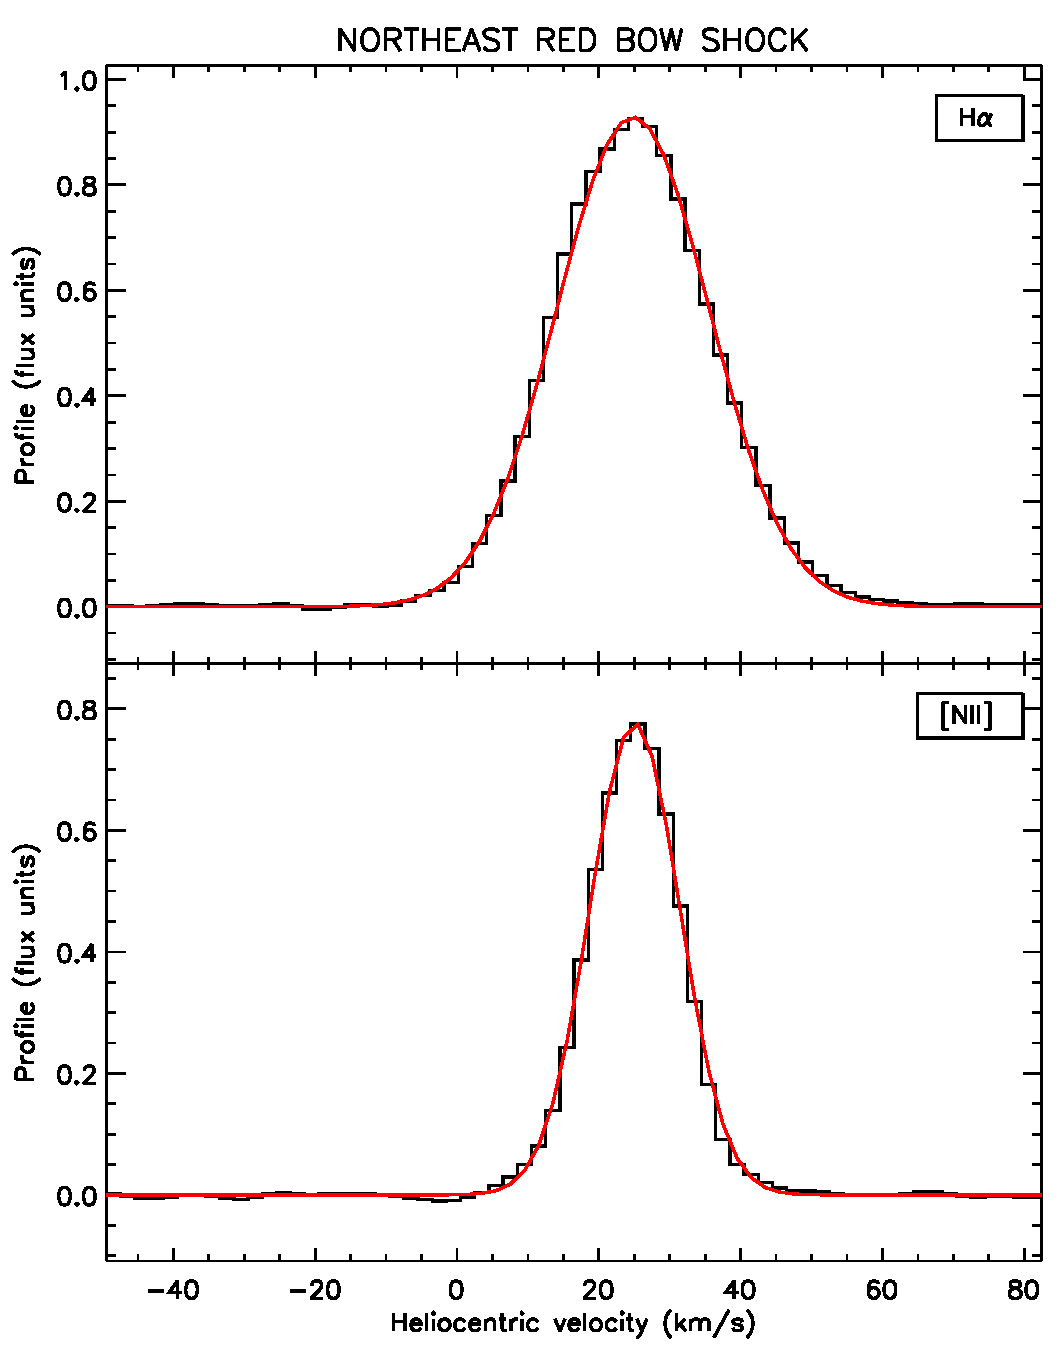
\includegraphics[width=\columnwidth]{Figs/redbowshockNE.pdf}  
    \caption{Spectral profiles in \Ha~(top) and \NII~(bottom) along the line of sight of the red bow-shock located to the northeast of the Wall. The black line 
    represents the profile extracted from the slit spectra after the core subtraction. The red line indicates the Gaussian fit performed.}
    \label{fig:red_fits}
\end{figure}


To estimate the velocity of the shocks we selected those slit positions which cross the bow-shocks in representative regions, if possible 
in areas close to the head of the bow. We found that no slit positions observed in \SII~or \OIII~are located near the bow-shocks, 
so we performed this study only in \Ha~and \NII~emission lines. One-dimensional spectra were extracted in the position of the shocks 
with an aperture of nine pixels. The thermal Doppler broadening of the line core (more relevant in \Ha~than in \NII) avoids to identify the 
profile of the shocks (with velocities around +20 \kms). For this reason, a subtraction of the line core was performed as a background. For each slit position
we extracted one-dimensional spectra in two representative regions which were combined by a mean to sample the background 
variations. These regions were selected as close to perpendicular to shock as possible and in areas outside the bow-shocks to avoid that 
the emission of the shocked gas dominates the spectrum. Once the line core was subtracted to all the one-dimensional spectra we 
performed Gaussian fits to the shock profiles weighted by the uncertainties of the background. Figure \ref{fig:red_fits} shows the spectral 
profile of one of the red bow-shocks (the northeast one) with the core subtraction and the Gaussian fit performed. All the fit performed worked 
well except for the NW shock where the background profile includes blueshifted emission near the line core making impossible to make a good 
subtraction on the blue side of the line.


Table \ref{table:redbowshocks_prop} lists the properties measured for the four red bow-shocks in \Ha~and \NII. Each studied shock is identified 
in the first column. The second and third columns give the heliocentric velocities measured for the centre of the Gaussian fits. Full width 
at half maximum (FWHM) are presented in columns 4 and 5, while fluxes obtained from the fits are shown in columns 6 and 7. The statistical errors 
associated with the measured fluxes were calculated integrating the residue of the fit over the whole velocity range of the line.\\




%-------------------------------------------TABLA: AJUSTES RED BOW SHOCKS---------------------------------------------------------------------------------------------------------
\begin{table}
\caption{Properties of the red bow-shocks detected in the western region of the Orion nebula.} 
\label{table:redbowshocks_prop} 
\centering 
\begin{tabular}{l c c c c c c }
\hline

Bow-shock    	&   \multicolumn{2}{c}{V$_{hel}$} &   \multicolumn{2}{c}{FWHM}    &  \multicolumn{2}{c}{Flux}         \\
				&   \multicolumn{2}{c}{(\kms)}    &   \multicolumn{2}{c}{(\kms)}  &  \multicolumn{2}{c}{(Flux units)}  \\
\hline
              		&      \Ha       &      \NII    &    \Ha        &      \NII     &      \Ha      			&   \NII             \\
\hline
NE				&	23.8	&	24.1	&	25.4	&	15.0	&	12.6$\pm$0.4	&	6.2$\pm$0.2	\\
NW$\dagger$	&	25.0	&	25.0	&	27.8		&	12.3	&	9.4$\pm$1.6		&	3.1$\pm$0.8	\\
SE				&	21.9	&	20.6	&	23.9	&	15.7	&	5.0$\pm$0.3		&	2.3$\pm$0.2	\\
SW-S			&	24.0	&	22.5	&	23.3	&	14.1	&	2.8$\pm$0.3		&	1.5$\pm$0.2	\\
SW-W			&	21.5	&	20.9	&	25.7	&	17.2		&	13.4$\pm$0.6	&	9.1$\pm$0.3	\\
\hline
\end{tabular}
\begin{list}{}{}\footnotesize{
\item $\dagger$ Bad subtraction of the line core.
}
\end{list}
\end{table}





%---------------------------------
%   4.2 MOVIMIENTOS PROPIOS
%---------------------------------
\subsection{Proper motions}\label{sec:propermotions}
The results shown in the previous section provide the velocity of the bow-shocks in our line of sight. However, to draw a tridimensional 
picture of the shock it is necessary to determine their velocity in the plane of the sky, i.e. to measure the proper motions.

With this aim a rough estimation of the proper motions of the large scale identified in our region was performed. We resorted to images 
of the western region of the Orion nebula observed with the ACS instrument of the HST which observations are separated almost 10 years. 
The first-epoch image was taken on April 26th 2005 while the second image was observed on March 2th 2015. The data used are calibrated 
and have a relative astrometric correction performed, however, to measure accurate displacements in the features we carry out an absolute 
astrometric calibration between both images.

We blink our matches images looking for nebular motions. In three of the five red bow shocks studied (NE, SW-S and SW-W).we find spatial 
displacement between the two epochs observed. In addition, we also detect clear motions in a little arc close to the SW-W red bow sock 
(identified as SW-W arc). For measurement, the profiles of the shocks were traced and compared in a manual mode. The displacements of 
the profiles between the two epochs were then measured. Taking into account that the time passed from the first epoch to the second is 
3957 days (3.10782$\times$10$^8$ seconds), we derived the velocity of each shock in the plane of the sky. Results are shown in Table \ref{table:propermotions}.




%-------------------------------------------TABLA: MOVIMIENTOS PROPIOS------------------------------------------------------------------------------
\begin{table}
\caption{Proper motions.} 
\label{table:propermotions} 
\centering 
\begin{tabular}{l c c c }
\hline

Bow-shock	&  V$_x$	&   V$_y$    	& V      \\
\hline
NE		&  $-$82	&  $-$101    	&  130   \\
SW-S		&  $-$97	&  $-$102    	&  141   \\
SW-W		&  $-$89	&  $-$112    	&  143   \\
SW-W arco	&  $-$96	&  $-$94	&  135   \\
\hline
\end{tabular}
\end{table}
%----------------------------------------------------------------------------------------------------------------------------------------------------






%%%%%%%%%%%%%%%%%%%%%%%%%%%%%%%%%%%%%%%%%%
%   5. KNOTS A ALTA VELOCIDAD
%%%%%%%%%%%%%%%%%%%%%%%%%%%%%%%%%%%%%%%%%%
\section{High-velocity knots}\label{sec:knots}

\begin{figure*}
    %\includegraphics[width=\textwidth]{Figs/rgb_blue_Ha.pdf} 
    \caption{\textbf{FIGURA POR HACER (WILL):} finding chart con knots identificados. Mejor zoom dejando 050-422 en una cajita.}  
    \label{fig:blue_features}
\end{figure*}


Analysing the position-velocity spectra and the isovelocity maps we detect five redshifted features at high-velocities located nearby to LL1 and LL2. All of them are 
already catalogued by \citet{Henney2013} and we do not perform any study of them in this work. On the other hand, we find \textbf{147} high-velocity 
blueshifted features in the isovelocity maps. They are distributed over the whole observation FoV, although, as can be appreciated in 
Fig. \ref{fig:blue_features}, there is a concentration of blueshifted knots to the south-west.\\
\textbf{Describir nuevo m�todo (WILL)}.Heliocentric velocities, FWHM and fluxes (with their corresponding errors) are presented in Table
\ref{table:blueknots_prop} for every detected blueshifted high-velocity feature in \Ha~and \NII. 




%-------------------------------------------TABLA: AJUSTES BLUE KNOTS---------------------------------------------------------------------------------------------------------
\onecolumn
%\begin{center}
\begin{longtable}{l c c c c c c c }
\caption{Heliocentric velocities, FWHM and fluxes for the blueshifted high-velocity knots studied in \Ha~and \NII.} \tabularnewline \hline
\label{table:blueknots_prop}
Knot  	& \multicolumn{2}{c}{V$_{hel}$} &   \multicolumn{2}{c}{FWHM}   &  \multicolumn{2}{c}{Flux}                \\
	& \multicolumn{2}{c}{(\kms)}    &   \multicolumn{2}{c}{(\kms)} &  \multicolumn{2}{c}{(Flux units)}    	 \\
	\hline \\
	 %\cline{4-12} \tabularnewline
			&       \Ha     &      \NII     &      \Ha      &        \NII  &        \Ha    		&        \NII       	\\
	\hline \\
	\endfirsthead
	\caption{Continued.} \\
	\hline
Knot  	& \multicolumn{2}{c}{V$_{hel}$} &   \multicolumn{2}{c}{FWHM}   &  \multicolumn{2}{c}{Flux}                \\
	& \multicolumn{2}{c}{(\kms)}    &   \multicolumn{2}{c}{(\kms)} &  \multicolumn{2}{c}{(Flux units)}    	 \\
	\hline \\
	 %\cline{4-12}
			&       \Ha     &      \NII     &      \Ha      &        \NII  &        \Ha    		&        \NII       	\\
	\hline  \\
	\endhead
	\\
 \hline	
  Continues. \\
	 \endfoot
	 \endlastfoot
 051-420   &   $-$30.00 $\pm$ 0.03   &     -   &    27.08 $\pm$ 1.58   &   -   &   9.98 $\pm$ 0.78   &   -  \\
 103-325   &     -   &   $-$32.79 $\pm$ 5.58   &     -   &  21.88 $\pm$ 8.71   &   -   &   2.49 $\pm$ 1.46  \\
4230-523   &   $-$30.00 $\pm$ 0.54   &   $-$30.00 $\pm$ 2.43   &    55.14 $\pm$ 3.65   &  58.87 $\pm$ 5.17   &   2.75 $\pm$ 0.55   &   0.91 $\pm$ 0.09  \\
4231-512   &   $-$30.00 $\pm$ 0.23   &   $-$35.76 $\pm$ 2.49   &    53.53 $\pm$ 4.30   &  29.62 $\pm$ 6.27   &   2.43 $\pm$ 0.22   &   0.51 $\pm$ 0.13  \\
4240-512   &   $-$55.73 $\pm$ 2.74   &   $-$48.22 $\pm$ 2.75   &    18.22 $\pm$ 5.35   &  23.75 $\pm$ 6.87   &   0.43 $\pm$ 0.16   &   0.44 $\pm$ 0.15  \\
4240-618   &   $-$20.00 $\pm$ 0.81   &   $-$20.00 $\pm$ 1.52   &    21.64 $\pm$ 4.36   &  58.35 $\pm$ 9.86   &   1.12 $\pm$ 0.27   &   0.93 $\pm$ 0.23  \\
4242-635   &    $-$8.38 $\pm$ 0.32   &    $-$2.99 $\pm$ 2.55   &    18.24 $\pm$ 0.85   &  15.16 $\pm$ 2.62   &   4.52 $\pm$ 0.23   &   1.13 $\pm$ 0.24  \\
4243-457   &   $-$17.36 $\pm$ 1.35   &   $-$20.06 $\pm$ 1.43   &    27.84 $\pm$ 2.34   &  19.34 $\pm$ 3.29   &   7.74 $\pm$ 2.94   &   2.37 $\pm$ 0.51  \\
4243-749   &   $-$67.49 $\pm$ 1.47   &   $-$68.21 $\pm$ 0.47   &    25.15 $\pm$ 3.26   &  33.33 $\pm$ 4.80   &   1.40 $\pm$ 0.17   &   0.75 $\pm$ 0.15  \\
4244-523   &   $-$68.02 $\pm$ 2.12   &   $-$70.75 $\pm$ 0.81   &    26.26 $\pm$ 3.30   &  19.57 $\pm$ 2.34   &   1.17 $\pm$ 0.29   &   0.26 $\pm$ 0.15  \\
4246-556   &   $-$99.26 $\pm$ 0.57   &   $-$94.79 $\pm$ 0.30   &    20.37 $\pm$ 1.21   &  24.95 $\pm$ 0.53   &   0.62 $\pm$ 0.00   &   0.67 $\pm$ 0.04  \\
4247-552   &   $-$66.70 $\pm$ 0.32   &   $-$66.41 $\pm$ 0.31   &    27.46 $\pm$ 0.78   &  15.00 $\pm$ 0.75   &   7.15 $\pm$ 0.25   &   3.63 $\pm$ 0.22  \\
4248-552   &   $-$10.49 $\pm$ 1.84   &   $-$14.47 $\pm$ 0.57   &    28.85 $\pm$ 1.41   &  18.18 $\pm$ 0.70   &  24.46 $\pm$ 2.49   &  10.54 $\pm$ 0.79  \\
4248-714   &    $-$6.06 $\pm$ 0.70   &    $-$5.04 $\pm$ 0.11   &    24.30 $\pm$ 1.51   &  11.78 $\pm$ 0.89   &   6.15 $\pm$ 0.39   &   0.47 $\pm$ 0.10  \\
4249-657   &   $-$11.94 $\pm$ 0.46   &   $-$13.86 $\pm$ 3.42   &    19.54 $\pm$ 1.29   &  28.22 $\pm$ 7.78   &   2.79 $\pm$ 0.21   &   0.34 $\pm$ 0.17  \\
4251-536   &   $-$70.43 $\pm$ 0.86   &   $-$70.78 $\pm$ 0.64   &    25.27 $\pm$ 0.84   &  14.86 $\pm$ 1.07   &   7.50 $\pm$ 1.68   &   2.78 $\pm$ 0.73  \\
4251-609   &   $-$78.52 $\pm$ 1.14   &   $-$81.22 $\pm$ 0.49   &    28.29 $\pm$ 1.46   &  19.80 $\pm$ 0.32   &   2.74 $\pm$ 1.33   &   1.21 $\pm$ 0.07  \\
4251-748   &   $-$64.85 $\pm$ 1.30   &   $-$70.12 $\pm$ 3.76   &    28.93 $\pm$ 2.93   &  39.05 $\pm$ 9.55   &   1.20 $\pm$ 0.15   &   0.85 $\pm$ 0.25  \\
4252-514   &   $-$64.04 $\pm$ 0.15   &   $-$70.00 $\pm$ 3.47   &    18.79 $\pm$ 4.24   &  42.26 $\pm$ 7.71   &   0.27 $\pm$ 0.11   &   0.46 $\pm$ 0.18  \\
4252-533   &    $-$8.13 $\pm$ 0.28   &    $-$9.30 $\pm$ 0.63   &    22.51 $\pm$ 0.69   &  16.22 $\pm$ 1.78   &   8.66 $\pm$ 0.28   &   1.90 $\pm$ 0.23  \\
4252-557   &   $-$69.67 $\pm$ 0.13   &   $-$69.81 $\pm$ 0.14   &    25.84 $\pm$ 0.33   &  14.57 $\pm$ 0.40   &  20.20 $\pm$ 3.56   &   8.98 $\pm$ 1.19  \\
4253-615   &   $-$12.54 $\pm$ 3.93   &   $-$15.79 $\pm$ 0.45   &    41.76 $\pm$ 2.68   &  26.08 $\pm$ 0.46   &  22.71 $\pm$12.37   &   3.96 $\pm$ 3.32  \\
4253-653   &   $-$77.73 $\pm$ 3.26   &     -   &    20.76 $\pm$ 7.15   &   -   &   0.31 $\pm$ 0.13   &   -  \\
4253-757   &   $-$58.81 $\pm$ 0.49   &   $-$60.12 $\pm$ 0.68   &    28.14 $\pm$ 1.31   &  26.61 $\pm$ 4.52   &   4.98 $\pm$ 1.63   &   2.12 $\pm$ 0.14  \\
4254-708   &   $-$59.44 $\pm$ 0.26   &   $-$57.76 $\pm$ 0.57   &    16.53 $\pm$ 3.23   &  12.84 $\pm$ 2.10   &   0.34 $\pm$ 0.13   &   0.20 $\pm$ 0.05  \\
4255-551   &   $-$67.91 $\pm$ 0.29   &   $-$68.98 $\pm$ 0.37   &    26.76 $\pm$ 0.67   &  17.66 $\pm$ 0.82   &  17.43 $\pm$ 2.73   &   7.46 $\pm$ 0.60  \\
4255-610   &   $-$63.25 $\pm$ 0.53   &   $-$62.93 $\pm$ 0.50   &    36.80 $\pm$ 2.07   &  30.99 $\pm$ 0.65   &  10.85 $\pm$ 1.07   &   5.17 $\pm$ 0.02  \\
4255-617   &   $-$95.58 $\pm$ 3.17   &  $-$100.00 $\pm$ 0.61   &    45.36 $\pm$ 5.84   &  14.94 $\pm$ 3.45   &   0.77 $\pm$ 0.19   &   0.19 $\pm$ 0.05  \\
4255-622   &   $-$61.77 $\pm$ 0.41   &   $-$62.18 $\pm$ 0.69   &    41.60 $\pm$ 0.94   &  33.73 $\pm$ 1.11   &  11.11 $\pm$ 1.29   &   6.43 $\pm$ 1.03  \\
4257-455   &   $-$49.83 $\pm$ 1.99   &   $-$54.75 $\pm$ 3.81   &    18.41 $\pm$ 0.32   &  24.74 $\pm$ 0.61   &   0.37 $\pm$ 0.08   &   0.32 $\pm$ 0.01  \\
4258-626   &   $-$60.76 $\pm$ 1.02   &   $-$59.26 $\pm$ 0.19   &    31.73 $\pm$ 1.43   &  27.35 $\pm$ 0.45   &  15.95 $\pm$ 1.25   &  11.59 $\pm$ 0.23  \\
4259-604   &   $-$14.52 $\pm$ 0.61   &   $-$14.12 $\pm$ 3.27   &    39.19 $\pm$ 4.25   &  58.87 $\pm$ 6.53   &   7.43 $\pm$ 0.81   &   2.24 $\pm$ 0.37  \\
4259-615   &   $-$61.09 $\pm$ 1.66   &   $-$56.23 $\pm$ 1.24   &    33.62 $\pm$ 1.88   &  21.29 $\pm$ 2.77   &  15.94 $\pm$ 4.05   &   8.13 $\pm$ 1.11  \\
4259-657   &    $-$7.04 $\pm$ 0.16   &    $-$4.92 $\pm$ 2.90   &    23.89 $\pm$ 0.35   &  34.62 $\pm$ 5.84   &  14.75 $\pm$ 0.22   &   5.64 $\pm$ 1.02  \\
4260-649   &   $-$25.16 $\pm$ 0.19   &   $-$25.00 $\pm$ 2.45   &    14.79 $\pm$ 1.58   &  39.56 $\pm$15.35   &   0.90 $\pm$ 0.26   &   1.69 $\pm$ 0.75  \\
4260-739   &   $-$61.39 $\pm$ 2.77   &   $-$63.78 $\pm$ 1.11   &    23.19 $\pm$ 0.02   &  19.65 $\pm$ 4.71   &   3.53 $\pm$ 0.86   &   1.24 $\pm$ 0.05  \\
4261-713   &   $-$55.79 $\pm$ 1.63   &   $-$54.34 $\pm$ 2.35   &    27.90 $\pm$ 0.69   &  16.97 $\pm$ 3.79   &   3.13 $\pm$ 0.95   &   0.98 $\pm$ 0.75  \\
4262-447   &   $-$25.30 $\pm$ 0.96   &   $-$34.51 $\pm$ 3.17   &    34.97 $\pm$ 6.91   &  17.22 $\pm$ 3.37   &   2.32 $\pm$ 0.72   &   0.59 $\pm$ 0.20  \\
4262-512   &   $-$60.37 $\pm$ 3.45   &   $-$64.19 $\pm$ 6.22   &    32.42 $\pm$ 7.95   &  39.20 $\pm$16.02   &   0.85 $\pm$ 0.26   &   0.52 $\pm$ 0.25  \\
4263-553   &   $-$61.28 $\pm$ 0.49   &   $-$61.24 $\pm$ 0.65   &    27.99 $\pm$ 0.24   &  19.15 $\pm$ 0.56   &  10.67 $\pm$ 0.34   &   3.04 $\pm$ 0.28  \\
4263-625   &   $-$56.34 $\pm$ 0.20   &   $-$58.45 $\pm$ 0.58   &    32.32 $\pm$ 0.68   &  31.71 $\pm$ 0.92   &  24.06 $\pm$ 2.78   &  13.30 $\pm$ 1.46  \\
4263-635   &   $-$51.60 $\pm$ 0.56   &   $-$47.17 $\pm$ 4.42   &    27.89 $\pm$ 0.17   &  19.64 $\pm$ 2.55   &   6.29 $\pm$ 0.60   &   0.18 $\pm$ 0.52  \\
4264-459   &   $-$35.00 $\pm$ 0.62   &   $-$37.67 $\pm$ 1.99   &    47.41 $\pm$ 1.81   &  15.16 $\pm$ 8.60   &   4.13 $\pm$ 0.35   &   0.22 $\pm$ 0.23  \\
4265-637   &   $-$12.53 $\pm$ 0.54   &   $-$15.00 $\pm$ 1.33   &    36.35 $\pm$ 1.77   &  29.91 $\pm$ 6.44   &   6.38 $\pm$ 0.31   &   1.15 $\pm$ 0.29  \\
4265-649   &   $-$39.57 $\pm$ 0.78   &   $-$51.83 $\pm$ 1.54   &    58.79 $\pm$ 0.18   &  18.80 $\pm$ 3.59   &  15.30 $\pm$ 0.25   &   1.11 $\pm$ 0.26  \\
4266-414   &   $-$51.84 $\pm$ 2.01   &   $-$52.96 $\pm$ 0.70   &    21.98 $\pm$ 1.60   &  15.06 $\pm$ 1.75   &   1.39 $\pm$ 0.60   &   0.27 $\pm$ 0.21  \\
4266-553   &   $-$10.21 $\pm$ 2.06   &    $-$7.81 $\pm$ 1.02   &    26.43 $\pm$ 1.50   &  22.43 $\pm$ 2.63   &  11.30 $\pm$ 1.78   &   4.10 $\pm$ 0.30  \\
4266-614   &   $-$51.33 $\pm$ 0.45   &   $-$54.49 $\pm$ 0.35   &    23.26 $\pm$ 0.72   &  15.87 $\pm$ 1.83   &  18.76 $\pm$ 2.28   &   5.51 $\pm$ 0.69  \\
4267-548   &   $-$64.49 $\pm$ 0.87   &   $-$64.73 $\pm$ 0.44   &    27.26 $\pm$ 0.10   &  16.66 $\pm$ 0.05   &  15.18 $\pm$ 0.79   &   5.21 $\pm$ 0.52  \\
4267-634   &   $-$59.22 $\pm$ 0.34   &   $-$59.03 $\pm$ 0.13   &    33.72 $\pm$ 1.29   &  27.71 $\pm$ 0.97   &   8.60 $\pm$ 3.02   &   3.41 $\pm$ 0.94  \\
4269-610   &    $-$7.42 $\pm$ 1.76   &    $-$4.89 $\pm$ 1.11   &    25.67 $\pm$ 3.19   &  20.47 $\pm$ 0.33   &  13.23 $\pm$ 2.52   &   4.28 $\pm$ 1.21  \\
4270-456   &   $-$15.53 $\pm$ 1.32   &   $-$26.18 $\pm$ 4.62   &    41.39 $\pm$ 2.30   &  46.35 $\pm$ 7.86   &   7.06 $\pm$ 0.99   &   1.51 $\pm$ 0.33  \\
4270-514   &    $-$9.96 $\pm$ 2.63   &    $-$9.44 $\pm$ 1.66   &    27.21 $\pm$ 1.79   &  18.90 $\pm$ 0.38   &   8.56 $\pm$ 1.45   &   1.68 $\pm$ 0.10  \\
4270-709   &   $-$55.75 $\pm$ 1.46   &     -   &    12.68 $\pm$ 1.67   &   -   &   1.13 $\pm$ 0.27   &   -  \\
4272-512   &   $-$52.99 $\pm$ 2.94   &     -   &    31.18 $\pm$ 6.05   &   -   &   1.32 $\pm$ 0.33   &   -  \\
4273-547   &   $-$63.02 $\pm$ 0.59   &   $-$63.13 $\pm$ 0.33   &    28.72 $\pm$ 0.41   &  19.65 $\pm$ 0.19   &  10.63 $\pm$ 3.40   &   5.89 $\pm$ 1.71  \\
4273-610   &   $-$62.92 $\pm$ 0.46   &   $-$65.27 $\pm$ 0.68   &    33.48 $\pm$ 1.82   &  24.07 $\pm$ 3.51   &   5.97 $\pm$ 0.46   &   1.65 $\pm$ 0.16  \\
4274-550   &    $-$7.16 $\pm$ 2.23   &    $-$9.17 $\pm$ 0.48   &    24.36 $\pm$ 1.76   &  18.38 $\pm$ 1.00   &  12.76 $\pm$ 1.82   &   2.54 $\pm$ 0.28  \\
4274-625   &   $-$44.56 $\pm$ 2.00   &   $-$54.57 $\pm$ 0.60   &    54.67 $\pm$ 1.49   &  23.74 $\pm$ 1.75   &   4.35 $\pm$ 1.31   &   2.09 $\pm$ 0.76  \\
4274-711   &   $-$35.00 $\pm$ 1.38   &   $-$37.81 $\pm$ 1.13   &    58.84 $\pm$ 0.09   &  49.33 $\pm$10.87   &   3.03 $\pm$ 0.75   &   0.86 $\pm$ 0.01  \\
4275-442   &   $-$60.03 $\pm$ 0.86   &   $-$62.20 $\pm$ 1.35   &    24.95 $\pm$ 1.14   &  16.19 $\pm$ 1.47   &   2.25 $\pm$ 0.43   &   0.81 $\pm$ 0.14  \\
4275-454   &   $-$30.00 $\pm$ 0.50   &   $-$30.15 $\pm$ 1.06   &    57.40 $\pm$ 4.81   &  55.13 $\pm$ 4.75   &   4.66 $\pm$ 1.09   &   1.18 $\pm$ 0.17  \\
4276-707   &    $-$4.99 $\pm$ 0.42   &    $-$9.60 $\pm$ 3.11   &    20.52 $\pm$ 0.88   &  21.93 $\pm$ 7.62   &   6.58 $\pm$ 0.29   &   0.52 $\pm$ 0.21  \\
4277-528   &    $-$7.48 $\pm$ 0.35   &    $-$4.00 $\pm$ 1.48   &    20.49 $\pm$ 1.47   &  16.46 $\pm$ 1.23   &  10.61 $\pm$ 1.07   &   3.15 $\pm$ 0.33  \\
4277-541   &   $-$76.78 $\pm$ 0.64   &   $-$77.31 $\pm$ 0.18   &    24.12 $\pm$ 1.44   &  12.60 $\pm$ 0.36   &   2.17 $\pm$ 0.16   &   0.51 $\pm$ 0.19  \\
4279-532   &   $-$64.80 $\pm$ 0.34   &   $-$63.69 $\pm$ 1.10   &    13.82 $\pm$ 2.90   &  14.71 $\pm$ 1.85   &   1.29 $\pm$ 0.54   &   0.22 $\pm$ 0.09  \\
4280-550   &   $-$66.73 $\pm$ 2.94   &   $-$69.84 $\pm$ 2.69   &    32.03 $\pm$ 1.51   &  20.63 $\pm$ 2.10   &   3.23 $\pm$ 0.65   &   0.84 $\pm$ 0.18  \\
4281-258   &   $-$11.47 $\pm$ 0.70   &   $-$22.28 $\pm$ 2.39   &    32.59 $\pm$ 1.78   &  31.70 $\pm$ 0.96   &   7.40 $\pm$ 0.42   &   9.91 $\pm$ 7.90  \\
4282-319   &   $-$12.91 $\pm$ 1.66   &   $-$24.64 $\pm$ 1.42   &    43.25 $\pm$ 4.53   &  28.04 $\pm$ 3.44   &  14.56 $\pm$12.73   &   3.41 $\pm$ 3.96  \\
4283-612   &   $-$31.50 $\pm$ 1.57   &   $-$38.84 $\pm$ 1.16   &    48.34 $\pm$ 2.27   &  27.00 $\pm$ 6.75   &   6.17 $\pm$ 0.55   &   1.06 $\pm$ 0.11  \\
4284-307   &   $-$20.18 $\pm$ 0.13   &   $-$26.21 $\pm$ 1.45   &    37.49 $\pm$ 1.20   &  27.29 $\pm$ 1.56   &  19.04 $\pm$ 4.90   &  12.55 $\pm$ 3.77  \\
4285-316   &   $-$30.00 $\pm$ 0.01   &   $-$31.40 $\pm$ 0.13   &    37.33 $\pm$ 0.45   &  29.36 $\pm$ 0.34   &  26.10 $\pm$ 0.35   &  13.84 $\pm$ 0.19  \\
4286-304   &   $-$12.74 $\pm$ 0.23   &    $-$5.97 $\pm$ 0.89   &    35.38 $\pm$ 0.79   &  49.44 $\pm$ 2.00   &  26.11 $\pm$ 0.59   &  17.59 $\pm$ 0.71  \\
4286-322   &   $-$24.88 $\pm$ 1.22   &   $-$29.43 $\pm$ 0.46   &    35.35 $\pm$ 1.05   &  21.49 $\pm$ 0.97   &  15.13 $\pm$ 0.36   &   6.48 $\pm$ 0.16  \\
4286-646   &   $-$20.00 $\pm$ 0.45   &   $-$20.00 $\pm$ 1.49   &    31.29 $\pm$ 4.45   &  29.07 $\pm$ 5.94   &   2.47 $\pm$ 0.40   &   0.78 $\pm$ 0.21  \\
4287-441   &   $-$58.93 $\pm$ 2.60   &   $-$61.80 $\pm$ 1.00   &    25.49 $\pm$ 2.02   &  18.44 $\pm$ 1.39   &   1.73 $\pm$ 0.07   &   0.50 $\pm$ 0.20  \\
4288-539   &   $-$67.80 $\pm$ 1.14   &   $-$67.68 $\pm$ 1.63   &    26.96 $\pm$ 2.77   &  12.33 $\pm$ 2.14   &   1.99 $\pm$ 0.25   &   0.46 $\pm$ 0.13  \\
4288-557   &   $-$64.00 $\pm$ 0.19   &   $-$62.30 $\pm$ 0.98   &    24.73 $\pm$ 0.32   &  13.42 $\pm$ 0.16   &   1.30 $\pm$ 0.46   &   0.38 $\pm$ 0.04  \\
4289-524   &   $-$68.81 $\pm$ 0.28   &   $-$71.27 $\pm$ 0.12   &    24.14 $\pm$ 1.39   &  15.74 $\pm$ 1.28   &   1.92 $\pm$ 0.32   &   0.40 $\pm$ 0.16  \\
4289-556   &   $-$21.77 $\pm$ 0.94   &   $-$30.11 $\pm$ 0.38   &    56.23 $\pm$ 3.08   &  32.91 $\pm$ 2.20   &   8.89 $\pm$ 3.59   &   1.80 $\pm$ 0.23  \\
4290-459   &    $-$7.97 $\pm$ 4.44   &    $-$8.29 $\pm$ 1.05   &    11.88 $\pm$ 0.61   &  14.46 $\pm$ 0.56   &  11.92 $\pm$ 1.69   &   4.51 $\pm$ 0.46  \\
4290-547   &    $-$9.32 $\pm$ 0.31   &    $-$9.98 $\pm$ 0.75   &    26.49 $\pm$ 7.14   &  12.51 $\pm$ 4.23   &   7.09 $\pm$ 2.02   &   1.21 $\pm$ 0.08  \\
4291-428   &   $-$14.75 $\pm$ 0.66   &   $-$10.00 $\pm$ 0.86   &    26.19 $\pm$ 1.81   &  37.33 $\pm$ 7.82   &   5.49 $\pm$ 0.43   &   1.81 $\pm$ 0.45  \\
4291-547   &   $-$65.38 $\pm$ 0.83   &   $-$73.10 $\pm$ 4.01   &    32.91 $\pm$ 1.98   &  49.39 $\pm$13.46   &   2.90 $\pm$ 0.21   &   0.49 $\pm$ 0.23  \\
4293-326   &   $-$13.02 $\pm$ 0.17   &     -   &    19.36 $\pm$ 0.47   &   -   &  11.04 $\pm$ 0.31   &   -  \\
4294-259   &   $-$30.00 $\pm$ 0.14   &     -   &    57.92 $\pm$ 3.92   &   -   &   3.52 $\pm$ 0.33   &   -  \\
4294-321   &   $-$52.54 $\pm$ 0.28   &   $-$53.29 $\pm$ 0.28   &    30.53 $\pm$ 0.66   &  21.93 $\pm$ 0.65   &   7.95 $\pm$ 0.21   &   5.13 $\pm$ 0.19  \\
4295-603   &   $-$64.75 $\pm$ 1.05   &   $-$52.50 $\pm$ 4.95   &    27.28 $\pm$ 0.76   &  58.87 $\pm$11.44   &   0.53 $\pm$ 0.14   &   0.33 $\pm$ 0.10  \\
4300-503   &    $-$7.46 $\pm$ 1.45   &    $-$6.97 $\pm$ 0.76   &    24.25 $\pm$ 1.34   &  19.55 $\pm$ 0.23   &  17.32 $\pm$ 4.53   &   3.90 $\pm$ 1.04  \\
4301-547   &   $-$70.20 $\pm$ 1.12   &   $-$73.50 $\pm$ 1.00   &    32.51 $\pm$ 2.67   &  11.77 $\pm$ 0.66   &   1.21 $\pm$ 0.12   &   0.09 $\pm$ 0.04  \\
4303-520   &   $-$52.44 $\pm$ 0.82   &   $-$58.53 $\pm$ 3.45   &    18.14 $\pm$ 2.63   &  16.35 $\pm$ 3.69   &   0.50 $\pm$ 0.06   &   0.12 $\pm$ 0.01  \\
4303-526   &   $-$16.67 $\pm$ 0.46   &   $-$15.00 $\pm$ 0.55   &    21.43 $\pm$ 1.22   &  28.11 $\pm$ 4.97   &   2.48 $\pm$ 0.17   &   0.67 $\pm$ 0.14  \\
4303-610   &   $-$35.00 $\pm$ 0.15   &     -   &    56.99 $\pm$ 6.77   &   -   &   2.55 $\pm$ 0.33   &   -  \\
4305-618   &   $-$61.92 $\pm$ 3.65   &   $-$68.99 $\pm$ 3.33   &    19.26 $\pm$ 5.76   &  50.17 $\pm$ 6.83   &   0.35 $\pm$ 0.15   &   0.68 $\pm$ 0.18  \\
4309-511   &   $-$56.74 $\pm$ 1.74   &   $-$62.79 $\pm$ 1.71   &    32.57 $\pm$ 2.19   &  45.49 $\pm$ 7.38   &   1.25 $\pm$ 0.23   &   0.34 $\pm$ 0.15  \\
4311-547   &   $-$25.00 $\pm$ 0.02   &   $-$25.00 $\pm$ 0.45   &    29.83 $\pm$ 0.83   &  44.71 $\pm$ 9.38   &   5.59 $\pm$ 0.18   &   0.82 $\pm$ 0.21  \\
4317-458   &   $-$12.94 $\pm$ 1.91   &    $-$9.04 $\pm$ 0.12   &    22.28 $\pm$ 0.75   &  21.31 $\pm$ 0.45   &   9.90 $\pm$ 2.22   &   2.75 $\pm$ 0.49  \\
4318-527   &   $-$25.00 $\pm$ 0.07   &   $-$30.37 $\pm$ 1.81   &    41.44 $\pm$ 3.03   &  11.77 $\pm$ 0.93   &   8.13 $\pm$ 0.63   &   0.19 $\pm$ 0.05  \\
4322-625   &   $-$64.67 $\pm$ 2.68   &   $-$64.84 $\pm$ 0.62   &    24.91 $\pm$ 0.74   &  15.19 $\pm$ 1.45   &   2.49 $\pm$ 1.38   &   0.83 $\pm$ 0.10  \\
4323-522   &   $-$12.53 $\pm$ 0.46   &   $-$10.00 $\pm$ 0.16   &    27.13 $\pm$ 1.46   &  29.94 $\pm$ 3.81   &   9.22 $\pm$ 0.54   &   2.11 $\pm$ 0.29  \\
4326-522   &   $-$63.92 $\pm$ 2.87   &     -   &    43.65 $\pm$11.92   &   -   &   0.55 $\pm$ 0.19   &   -  \\
4328-601   &   $-$60.16 $\pm$ 3.86   &     -   &    12.90 $\pm$ 3.23   &   -   &   0.25 $\pm$ 0.13   &   -  \\
4333-355   &   $-$15.25 $\pm$ 0.32   &     -   &    17.75 $\pm$ 1.79   &   -   &   2.50 $\pm$ 0.30   &   -  \\
4333-403   &   $-$65.57 $\pm$ 2.29   &   $-$65.45 $\pm$ 2.60   &    16.85 $\pm$ 3.16   &  18.21 $\pm$ 5.73   &   0.86 $\pm$ 0.27   &   0.74 $\pm$ 0.29  \\
4334-456   &   $-$15.03 $\pm$ 0.19   &   $-$15.00 $\pm$ 0.09   &    30.39 $\pm$ 1.42   &  24.17 $\pm$ 1.52   &  15.99 $\pm$ 2.45   &   3.50 $\pm$ 0.34  \\
4337-210   &     -   &   $-$19.53 $\pm$ 0.03   &     -   &  16.17 $\pm$ 0.07   &   -   &  56.33 $\pm$ 0.29  \\
4338-514   &   $-$48.37 $\pm$ 5.03   &     -   &    33.71 $\pm$ 7.54   &   -   &   0.26 $\pm$ 0.14   &   -  \\
4344-512   &    $-$7.43 $\pm$ 0.94   &    $-$3.46 $\pm$ 0.44   &    24.52 $\pm$ 1.60   &  17.75 $\pm$ 1.27   &  20.75 $\pm$ 4.43   &   5.40 $\pm$ 2.16  \\
4356-525   &   $-$28.56 $\pm$ 0.35   &   $-$36.69 $\pm$ 1.04   &    38.07 $\pm$ 1.37   &  15.25 $\pm$ 0.54   &   8.41 $\pm$ 0.98   &   0.85 $\pm$ 0.17  \\
4363-514   &   $-$35.00 $\pm$ 0.15   &   $-$44.40 $\pm$ 0.74   &    53.87 $\pm$ 3.83   &  11.92 $\pm$ 0.90   &   4.37 $\pm$ 0.36   &   0.35 $\pm$ 0.05  \\
4368-523   &   $-$96.17 $\pm$ 7.14   &   $-$93.08 $\pm$ 4.36   &    18.41 $\pm$ 7.58   &  28.19 $\pm$21.34   &   0.10 $\pm$ 0.08   &   0.12 $\pm$ 0.11  \\
4374-457   &   $-$68.60 $\pm$ 5.27   &     -   &    33.26 $\pm$ 8.40   &   -   &   0.58 $\pm$ 0.35   &   -  \\
4377-210   &    $-$7.06 $\pm$ 1.85   &   $-$10.71 $\pm$ 1.80   &    25.36 $\pm$ 0.98   &  16.64 $\pm$ 3.34   &  21.93 $\pm$ 5.82   &   2.35 $\pm$ 0.62  \\
4378-230   &   $-$60.63 $\pm$ 3.16   &     -   &    23.08 $\pm$ 7.58   &   -   &   0.49 $\pm$ 0.20   &   -  \\
4378-526   &   $-$70.20 $\pm$ 0.43   &   $-$71.07 $\pm$ 1.23   &    31.47 $\pm$ 1.64   &  13.60 $\pm$ 1.80   &   1.35 $\pm$ 0.39   &   0.12 $\pm$ 0.08  \\
4380-337   &   $-$64.21 $\pm$ 1.05   &   $-$62.95 $\pm$ 3.89   &    35.22 $\pm$ 2.66   &  16.94 $\pm$ 4.49   &   2.05 $\pm$ 0.19   &   0.29 $\pm$ 0.13  \\
4380-343   &    $-$9.76 $\pm$ 0.32   &    $-$5.00 $\pm$ 0.82   &    21.48 $\pm$ 0.93   &  32.45 $\pm$ 3.39   &   5.06 $\pm$ 0.24   &   2.05 $\pm$ 0.24  \\
4380-417   &   $-$81.37 $\pm$ 1.90   &   $-$87.02 $\pm$ 3.56   &    17.12 $\pm$ 4.53   &  11.77 $\pm$ 8.09   &   0.29 $\pm$ 0.10   &   0.14 $\pm$ 0.11  \\
4380-519   &   $-$47.07 $\pm$ 2.85   &     -   &    32.75 $\pm$ 0.73   &   -   &   0.84 $\pm$ 0.36   &   -  \\
4381-409   &   $-$69.19 $\pm$ 2.37   &   $-$66.01 $\pm$ 1.71   &    30.23 $\pm$ 7.53   &  18.79 $\pm$ 5.37   &   1.18 $\pm$ 0.69   &   0.18 $\pm$ 0.04  \\
4381-438   &   $-$62.37 $\pm$ 4.57   &     -   &    18.07 $\pm$ 4.38   &   -   &   0.47 $\pm$ 0.23   &   -  \\
4381-442   &     -   &    $-$2.30 $\pm$ 0.45   &     -   &  19.01 $\pm$ 0.75   &   -   &   6.20 $\pm$ 0.25  \\
4381-455   &   $-$12.08 $\pm$ 0.10   &     1.80 $\pm$ 0.91   &    14.32 $\pm$ 0.27   &  11.77 $\pm$ 0.72   &   7.31 $\pm$ 0.16   &   4.44 $\pm$ 0.56  \\
4381-552   &  $-$100.19 $\pm$ 1.19   &   $-$93.65 $\pm$ 1.63   &    21.76 $\pm$ 3.78   &  29.73 $\pm$ 0.57   &   0.24 $\pm$ 0.07   &   0.26 $\pm$ 0.04  \\
4382-328   &   $-$79.75 $\pm$ 1.59   &   $-$79.79 $\pm$ 3.23   &    20.07 $\pm$ 1.66   &  12.76 $\pm$ 3.36   &   0.79 $\pm$ 0.55   &   0.31 $\pm$ 0.09  \\
4387-223   &    $-$6.39 $\pm$ 0.85   &    $-$1.13 $\pm$ 2.26   &    23.01 $\pm$ 0.88   &  25.25 $\pm$ 5.45   &  17.85 $\pm$ 1.15   &   2.61 $\pm$ 0.63  \\
4387-340   &   $-$63.57 $\pm$ 1.40   &   $-$66.62 $\pm$ 1.23   &    23.48 $\pm$ 3.50   &  22.53 $\pm$ 2.77   &   1.14 $\pm$ 0.39   &   0.28 $\pm$ 0.07  \\
4389-209   &    $-$6.32 $\pm$ 0.51   &    $-$5.22 $\pm$ 0.90   &    21.35 $\pm$ 0.88   &  16.21 $\pm$ 0.41   &  18.99 $\pm$ 1.03   &   2.48 $\pm$ 0.28  \\
4390-142   &    $-$9.61 $\pm$ 0.16   &    $-$6.06 $\pm$ 0.20   &    19.06 $\pm$ 0.60   &  15.23 $\pm$ 0.19   &  20.04 $\pm$ 0.41   &   4.39 $\pm$ 0.08  \\
4390-326   &   $-$75.00 $\pm$ 0.89   &   $-$83.06 $\pm$ 5.34   &    35.60 $\pm$ 7.60   &  36.57 $\pm$10.42   &   0.79 $\pm$ 0.23   &   0.29 $\pm$ 0.17  \\
4390-457   &   $-$71.41 $\pm$ 2.92   &     -   &    11.77 $\pm$13.91   &   -   &   0.09 $\pm$ 0.12   &   -  \\
4391-419   &   $-$67.07 $\pm$ 5.25   &     -   &    22.68 $\pm$ 9.22   &   -   &   0.26 $\pm$ 0.14   &   -  \\
4392-231   &   $-$75.20 $\pm$ 1.51   &   $-$78.11 $\pm$ 3.04   &    18.93 $\pm$ 1.91   &  12.46 $\pm$ 9.94   &   0.47 $\pm$ 0.11   &   0.15 $\pm$ 0.15  \\
4397-356   &   $-$68.92 $\pm$ 4.18   &     -   &    20.06 $\pm$ 6.50   &   -   &   0.47 $\pm$ 0.22   &   -  \\
4397-544   &   $-$88.21 $\pm$ 0.47   &   $-$89.34 $\pm$ 0.38   &    21.53 $\pm$ 1.11   &  23.09 $\pm$ 3.28   &   0.82 $\pm$ 0.14   &   0.40 $\pm$ 0.05  \\
4398-305   &   $-$61.73 $\pm$ 2.02   &   $-$55.05 $\pm$ 2.56   &    11.77 $\pm$ 3.63   &  11.77 $\pm$16.60   &   0.23 $\pm$ 0.17   &   0.28 $\pm$ 0.43  \\
4399-305   &     2.25 $\pm$ 0.13   &     3.92 $\pm$ 0.93   &    11.77 $\pm$ 0.05   &  21.99 $\pm$ 1.15   &  15.20 $\pm$ 0.41   &   4.29 $\pm$ 0.31  \\
4399-332   &   $-$70.52 $\pm$ 0.01   &   $-$59.09 $\pm$ 6.94   &    18.91 $\pm$ 0.16   &  12.56 $\pm$16.02   &   0.70 $\pm$ 0.11   &   0.09 $\pm$ 0.14  \\
4402-526   &   $-$89.98 $\pm$ 1.31   &   $-$94.12 $\pm$ 0.02   &    19.46 $\pm$ 1.59   &  25.27 $\pm$ 0.43   &   0.21 $\pm$ 0.08   &   0.18 $\pm$ 0.02  \\
4406-246   &   $-$68.11 $\pm$ 0.80   &   $-$70.98 $\pm$ 4.43   &    22.16 $\pm$ 2.36   &  11.77 $\pm$ 3.71   &   1.11 $\pm$ 0.21   &   0.17 $\pm$ 0.03  \\
4406-345   &   $-$71.86 $\pm$ 1.90   &   $-$76.16 $\pm$ 1.32   &    23.43 $\pm$ 3.11   &  13.46 $\pm$ 0.91   &   0.73 $\pm$ 0.24   &   0.28 $\pm$ 0.04  \\
4406-514   &   $-$72.68 $\pm$ 5.19   &   $-$75.67 $\pm$ 3.03   &    31.83 $\pm$10.39   &  11.77 $\pm$ 8.92   &   0.55 $\pm$ 0.23   &   0.09 $\pm$ 0.10  \\
4407-259   &  $-$122.94 $\pm$ 2.68   &  $-$125.00 $\pm$ 3.98   &    34.81 $\pm$10.38   &  56.99 $\pm$ 8.57   &   0.24 $\pm$ 0.06   &   0.64 $\pm$ 0.20  \\
4417-354   &   $-$24.33 $\pm$ 0.65   &   $-$15.00 $\pm$ 0.28   &    15.55 $\pm$ 1.45   &  18.43 $\pm$ 4.95   &   1.89 $\pm$ 0.22   &   0.49 $\pm$ 0.16  \\
4457-321   &   $-$68.52 $\pm$ 1.35   &   $-$75.00 $\pm$ 4.61   &    18.41 $\pm$ 0.46   &  12.30 $\pm$20.68   &   3.52 $\pm$ 1.15   &   1.25 $\pm$ 2.10  \\
\hline	
\end{longtable}
\twocolumn





%%%%%%%%%%%%%%%%%%%%%%%%%%%%%%%%%%%%%%%%%%
%   6 DISCUSION
%%%%%%%%%%%%%%%%%%%%%%%%%%%%%%%%%%%%%%%%%%
\section{Discussion}\label{sec:discussion}
The isovelocity maps and the 2D spectra reveal many new features which have been kinematically described in the previous sections. 
Now, we will interpret these results to \textbf{...}.





% ------------------------------
% 6.1 DISCUSION RED BOW SHOCKS
% ------------------------------
\subsection{Discusion red bow-shocks}\label{sec:disc_bowshocks}
\renewcommand{\labelenumi}{$\bullet$}
\begin{enumerate}
 \item Decir que son los bow shocks mas grandes vistos en Orion hasta ahora.
 \item Edad dinamica (necesario mopvimientos propios).
 \item Tasa de perdida de masa.
 \item Discutir el origen de los flujos.
\end{enumerate}









% -----------------------------------
% 6.2 ESTADISTICAS DE LOS BLUE KNOTS
% -----------------------------------
\subsection{Blue knots classification}\label{sec:blueknots_classification}
Estadisticas de los knots. Figuras provisionales


\begin{figure*}
    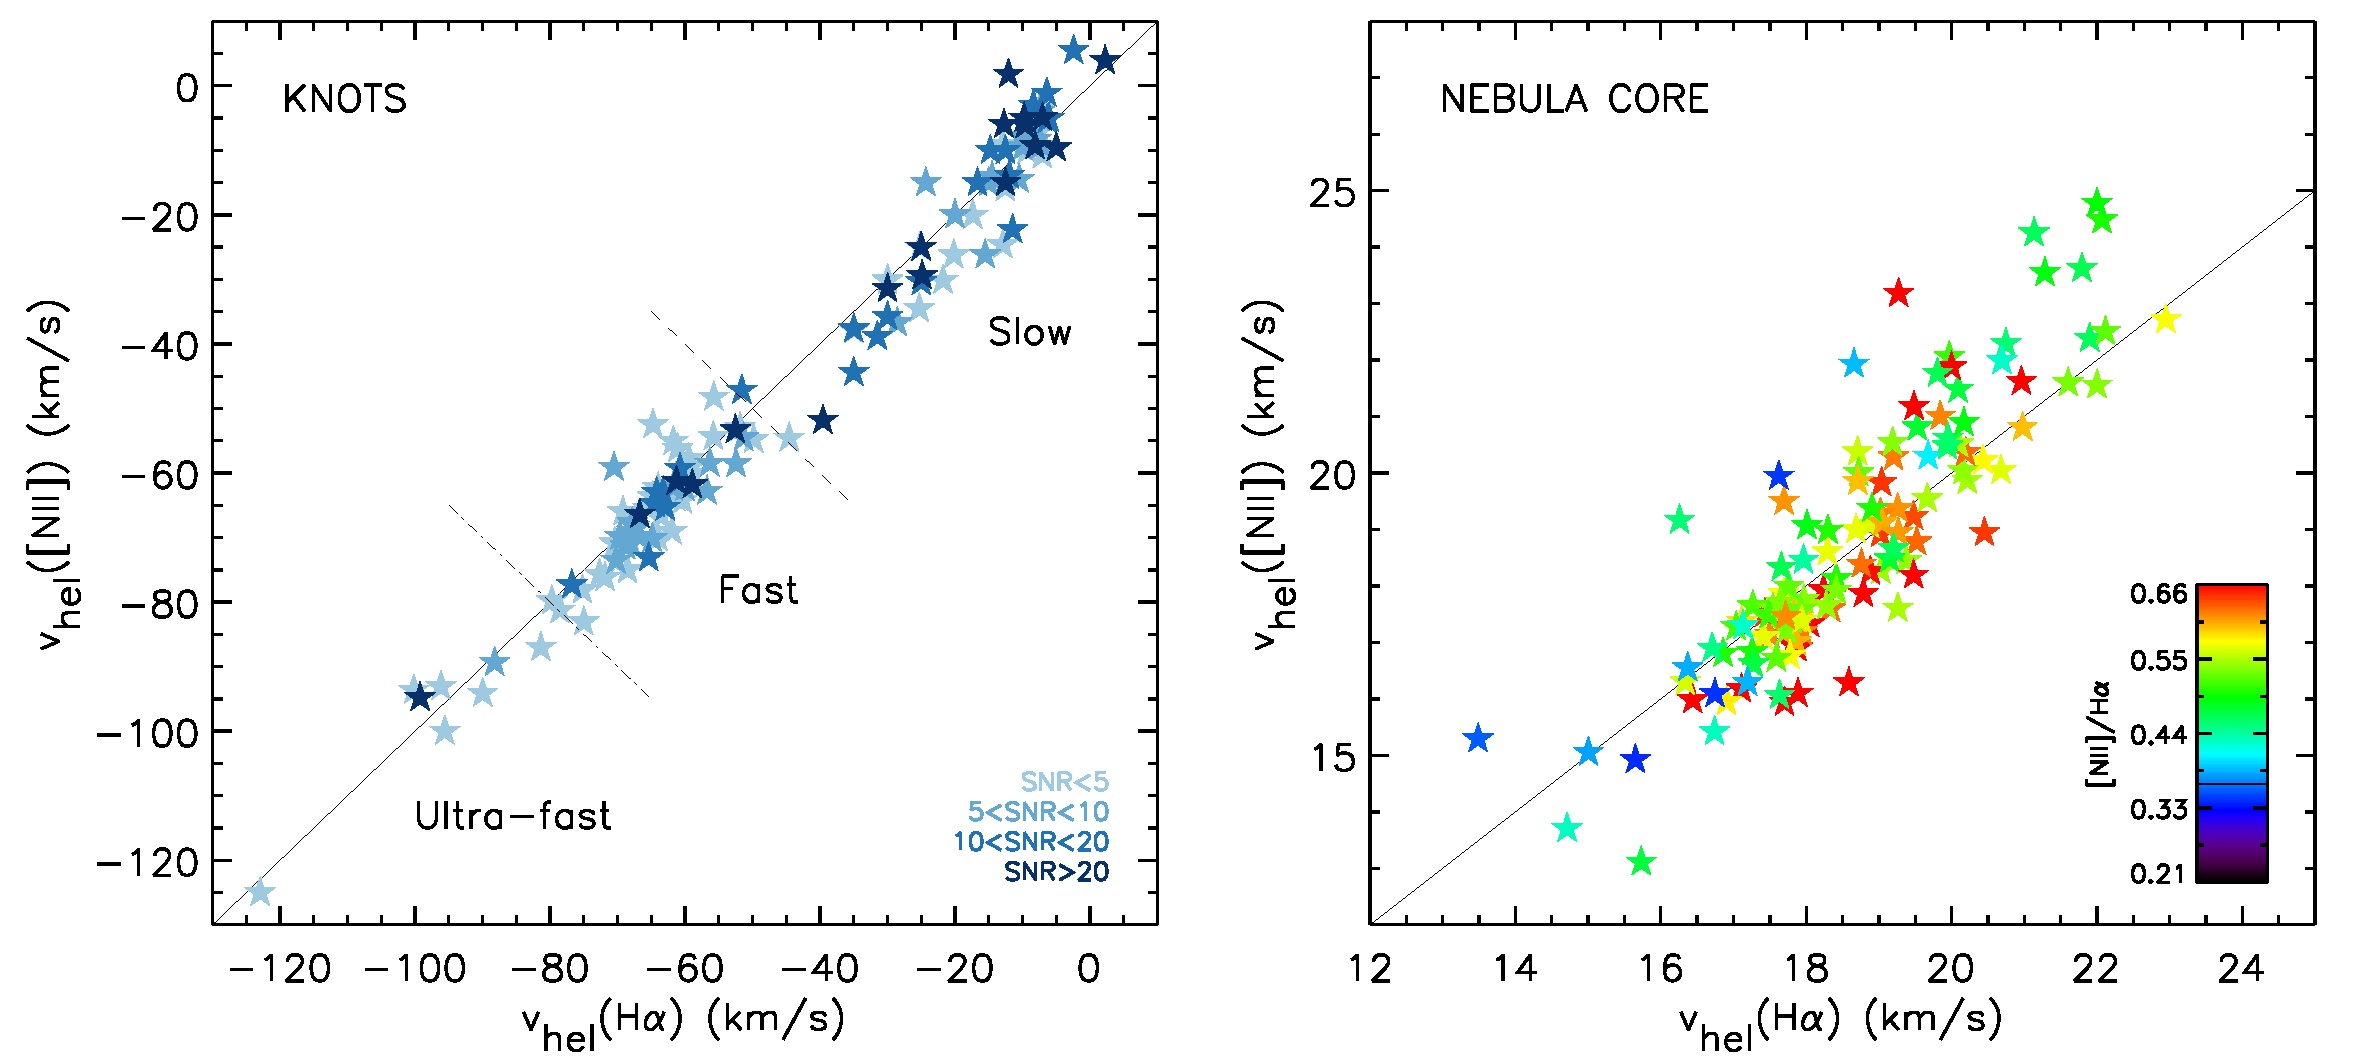
\includegraphics[width=\textwidth]{Figs/prov/Vnii_Vha.pdf} 
    \caption{Estadisticas1. Provisional}
    \label{fig:blue_stad}
\end{figure*}

\begin{figure}
  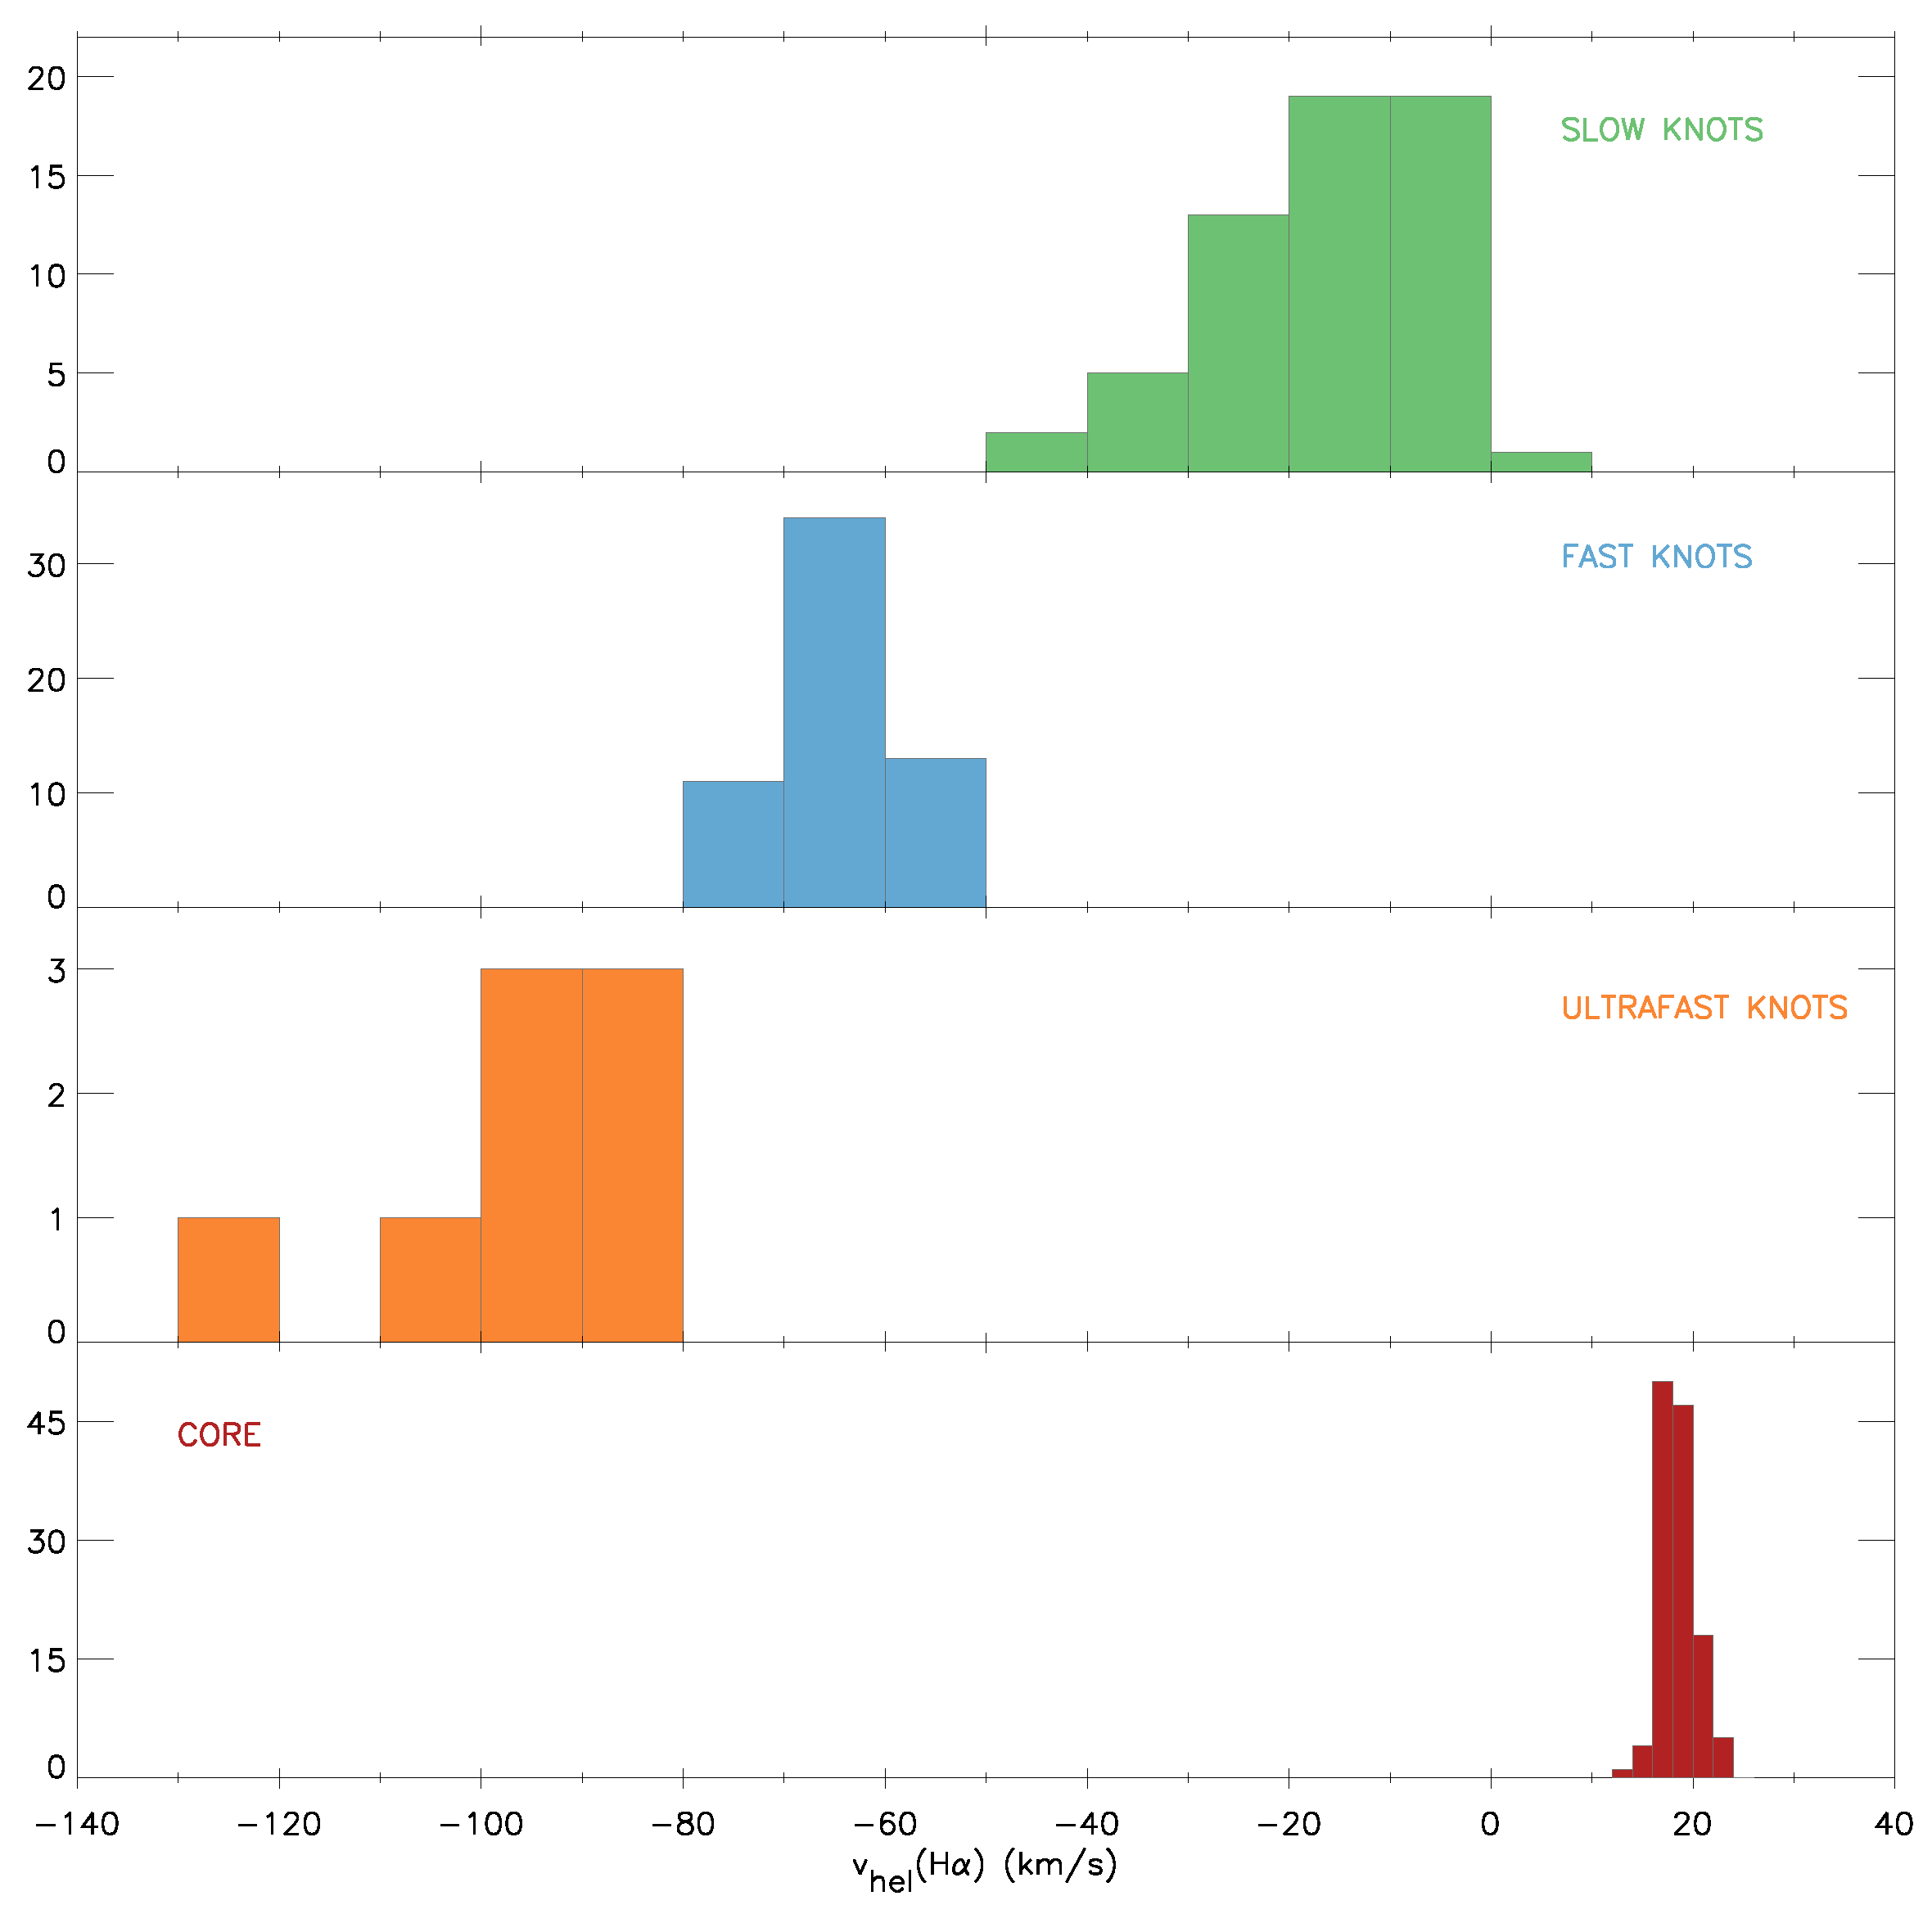
\includegraphics[width=\columnwidth]{Figs/prov/Hist_vHa.pdf} 
    \caption{Estadisticas2. Provisional}
\end{figure}

\begin{figure}
    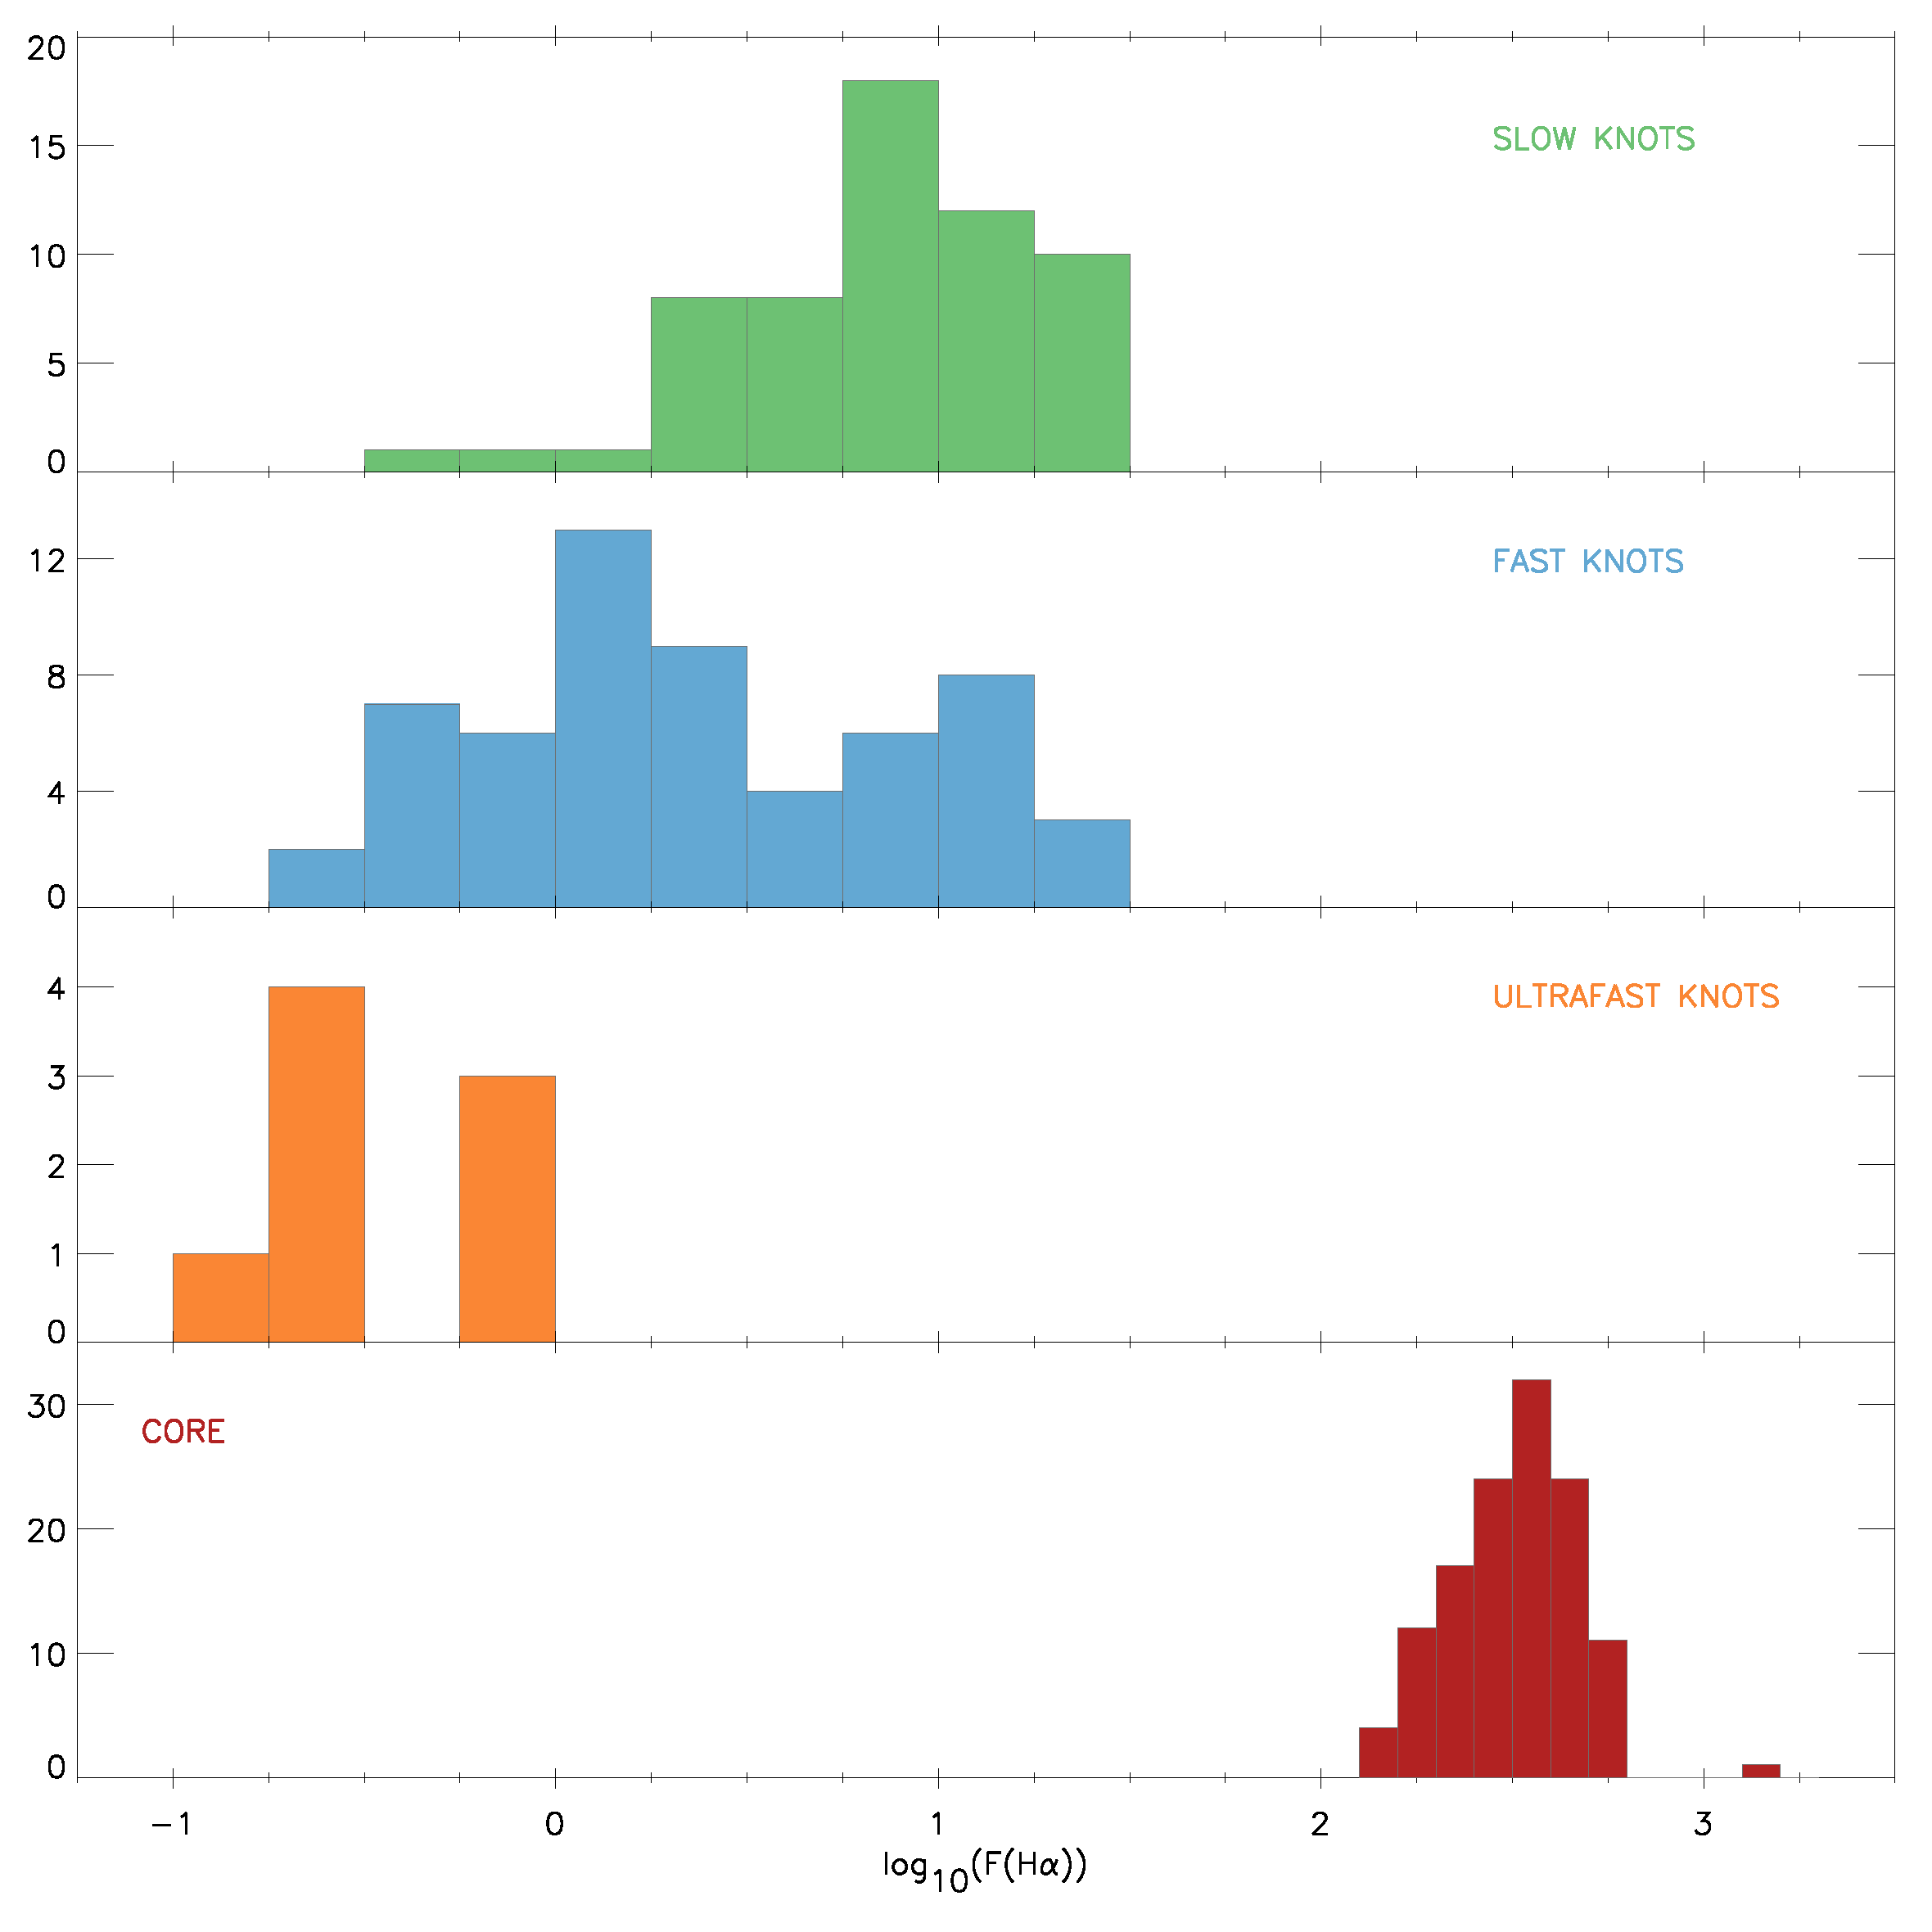
\includegraphics[width=\columnwidth]{Figs/prov/Hist_FHa.pdf} 
    \caption{Estadisticas3. Provisional}
\end{figure}

\begin{figure}
    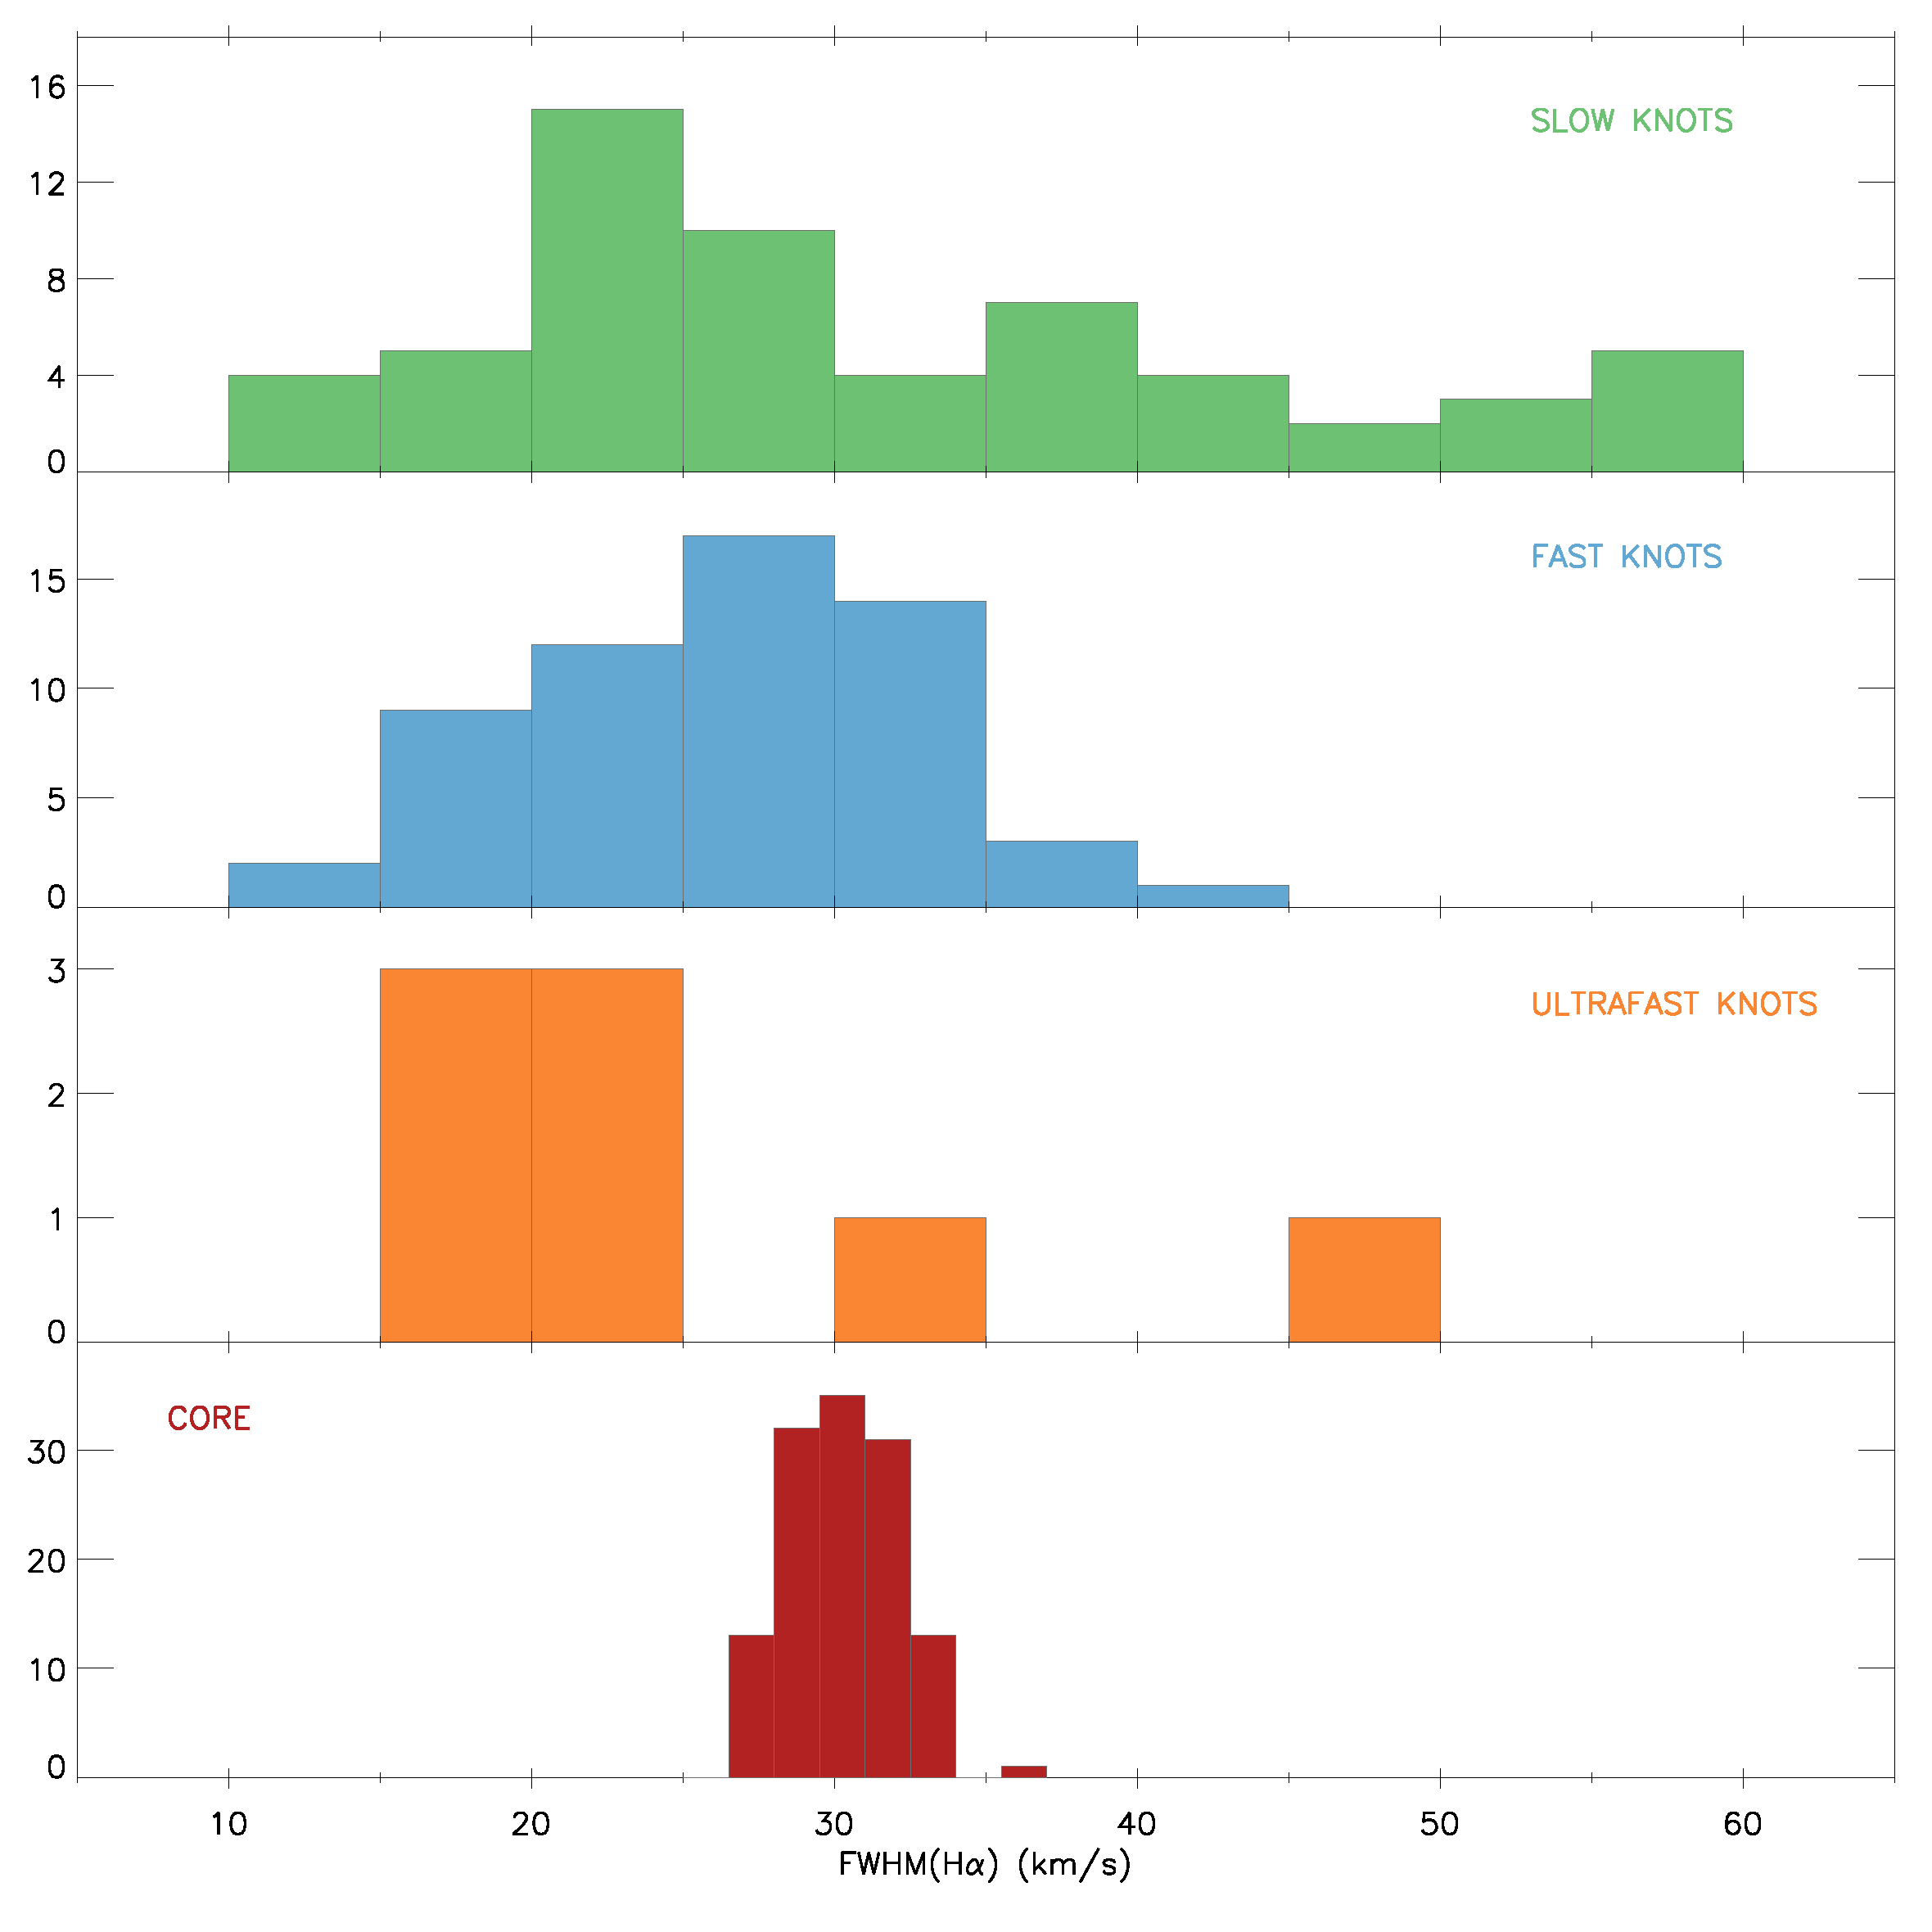
\includegraphics[width=\columnwidth]{Figs/prov/Hist_FWHM_Ha.pdf} 
    \caption{Estadisticas4. Provisional}
\end{figure}

\begin{figure}
   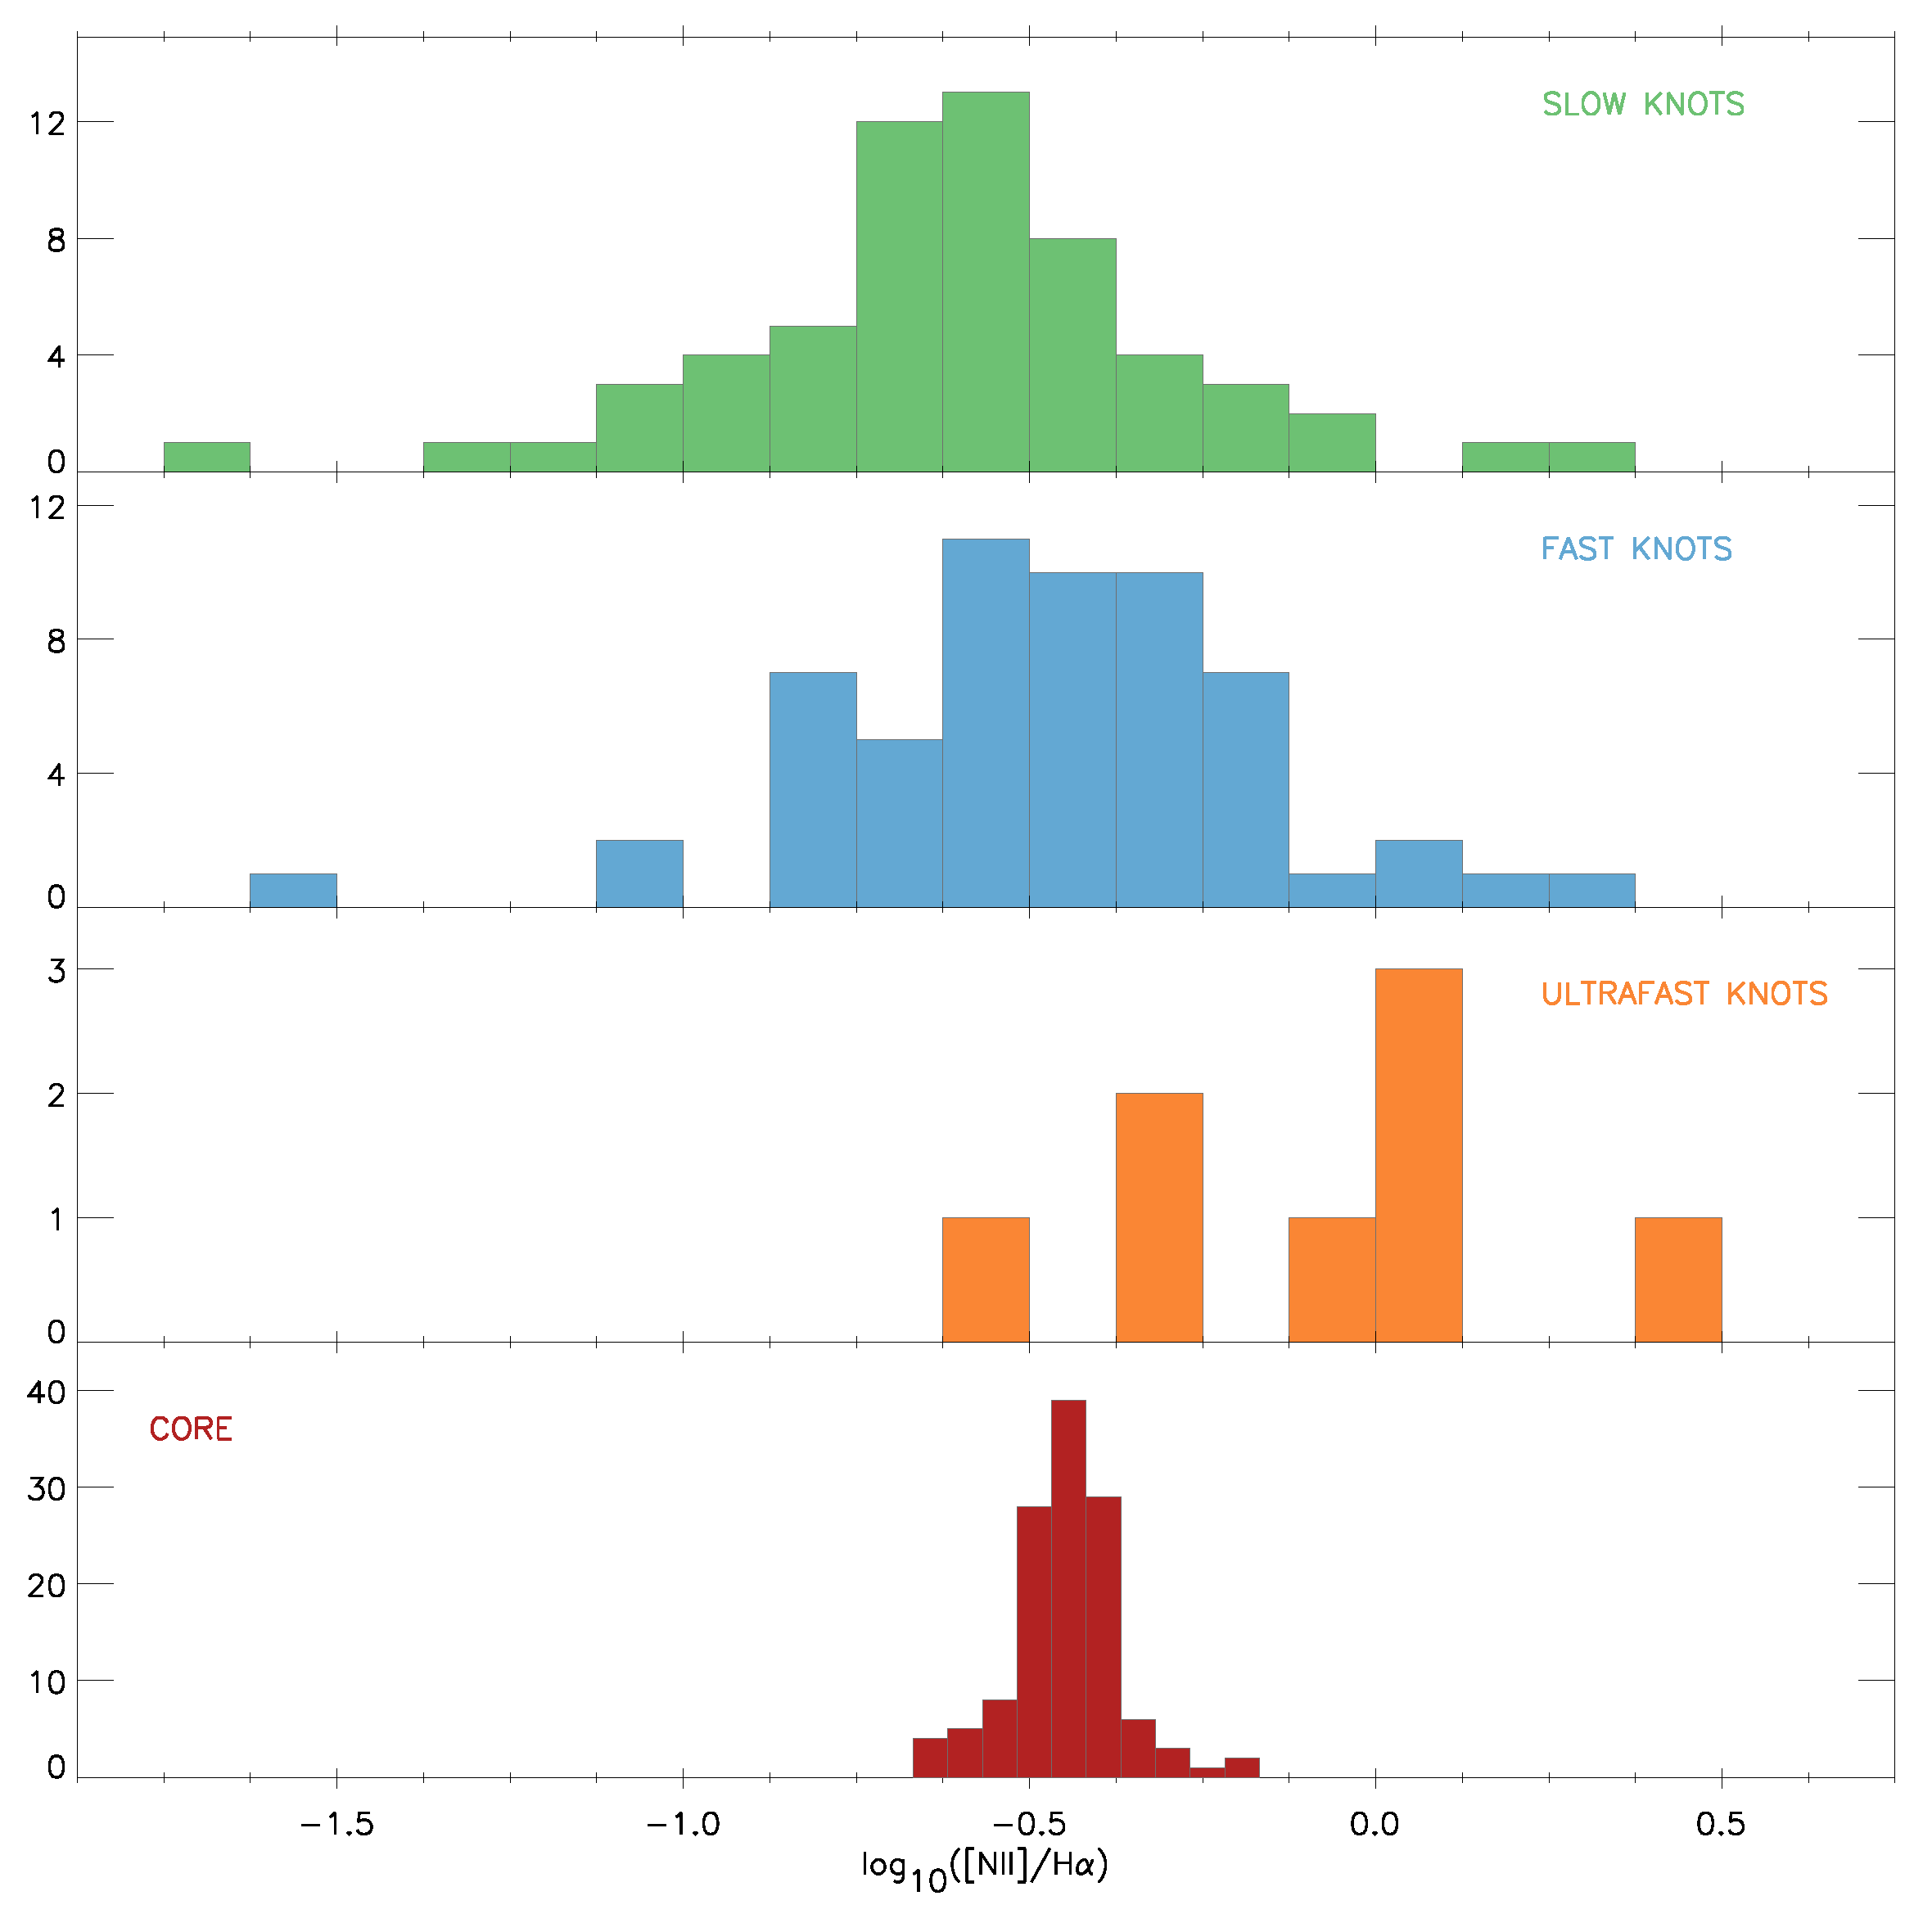
\includegraphics[width=\columnwidth]{Figs/prov/Hist_NIIHa.pdf} 
    \caption{Estadisticas5. Provisional}
\end{figure}

\begin{figure}
   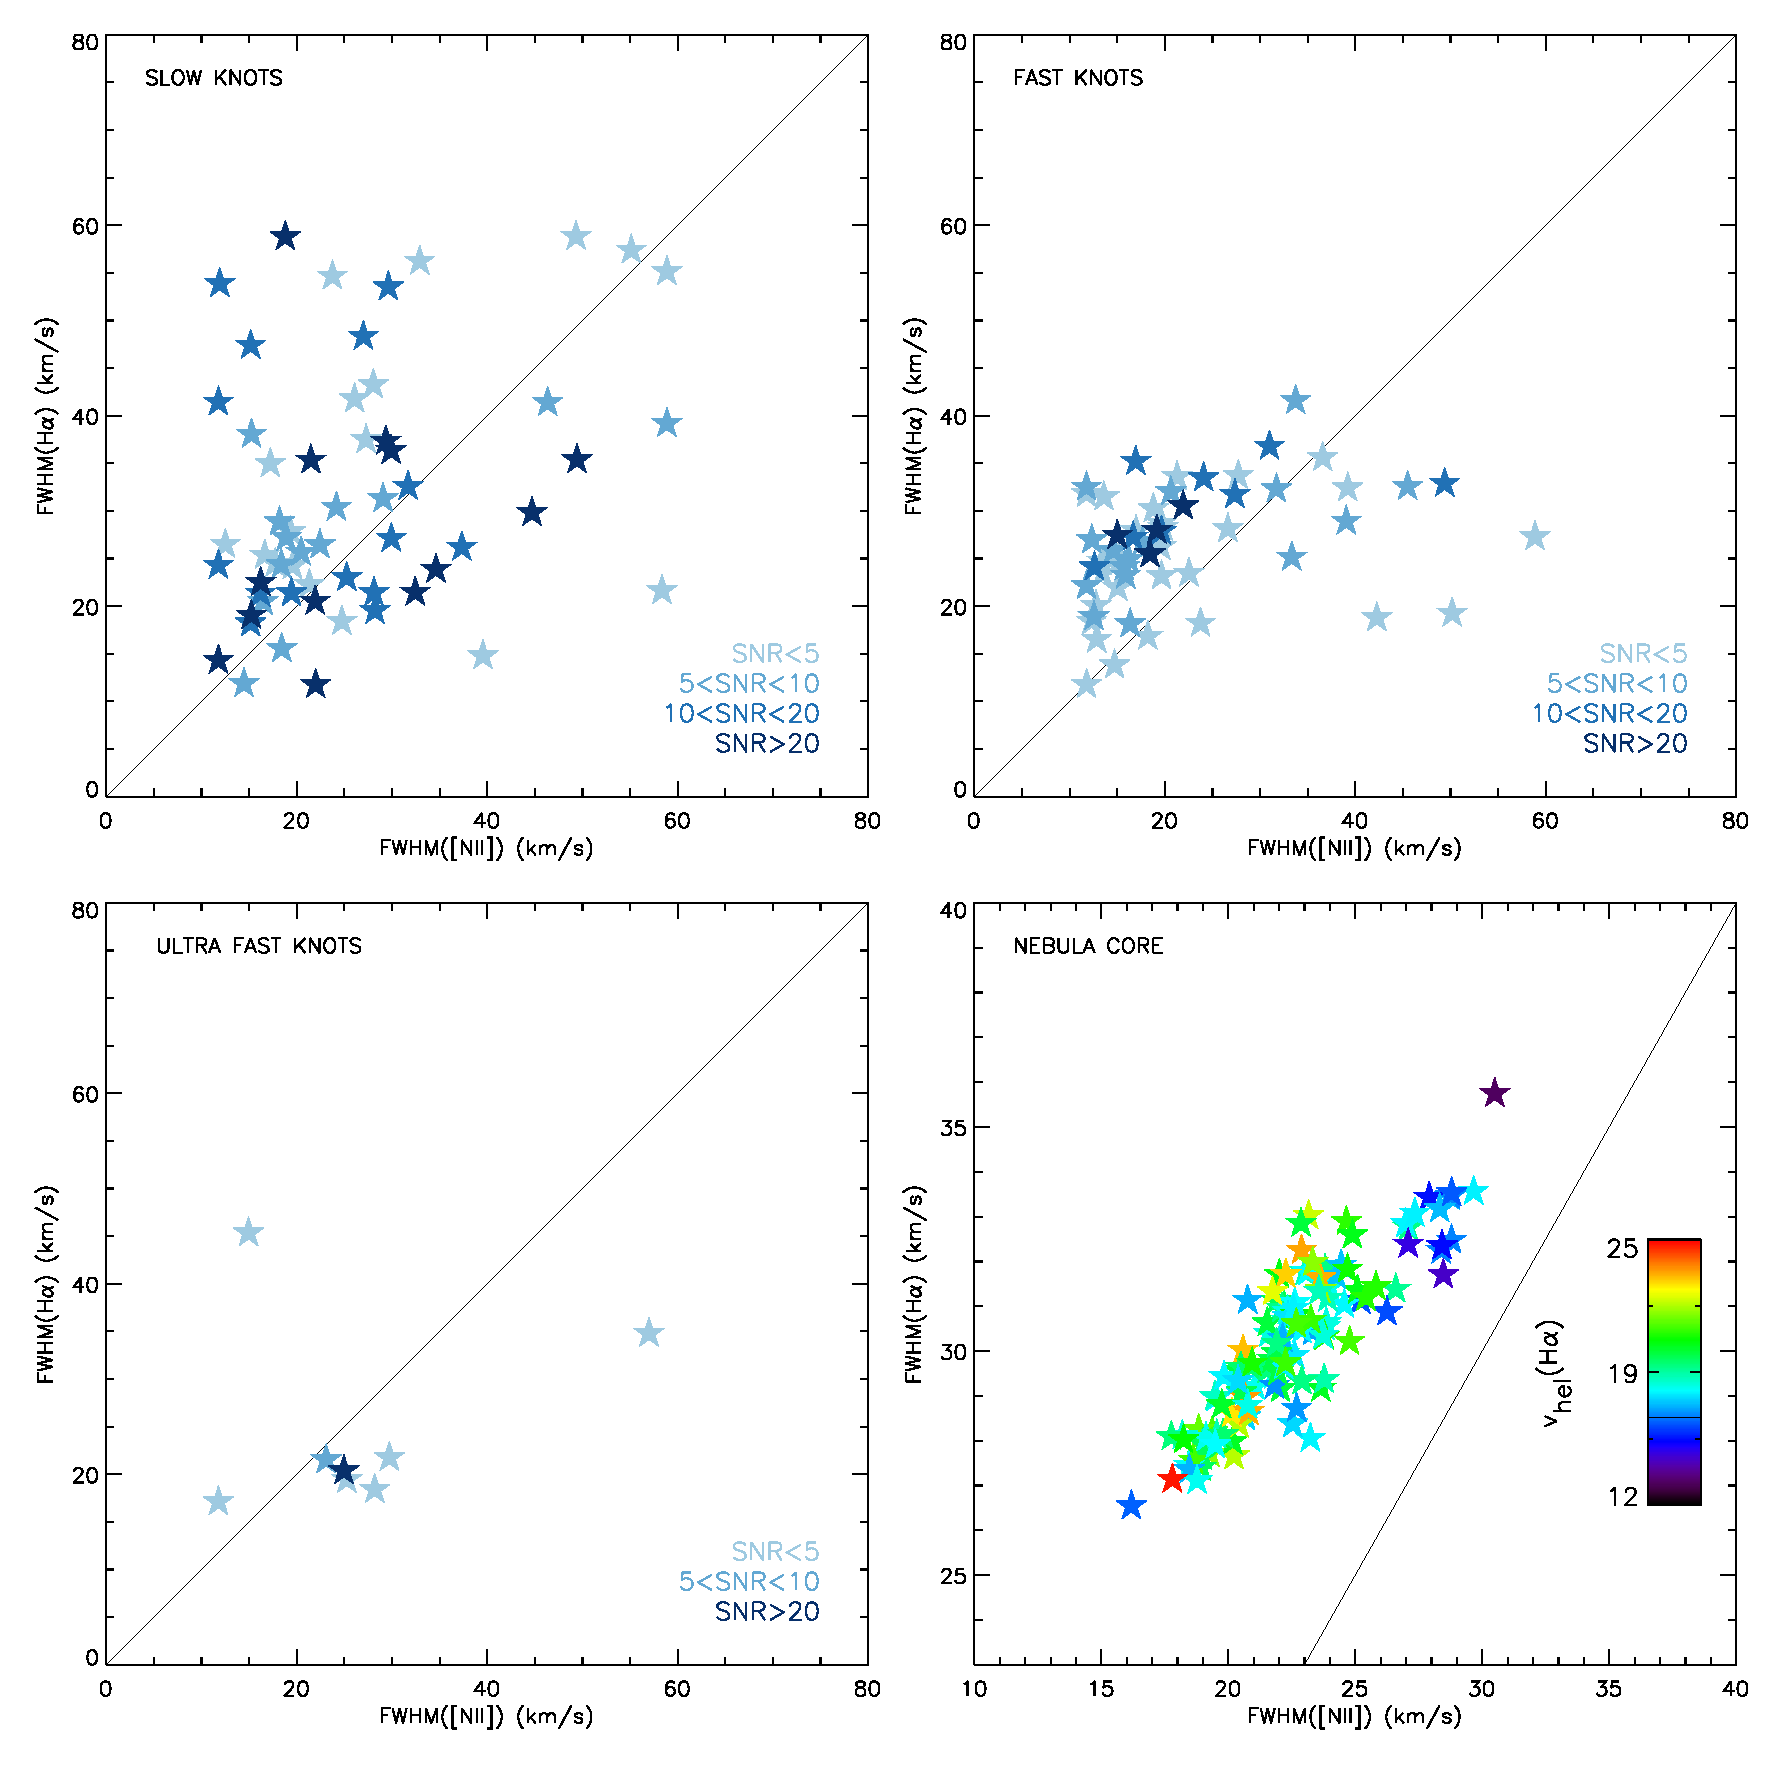
\includegraphics[width=\columnwidth]{Figs/prov/WHa_WNII.pdf} 
    \caption{Estadisticas6. Provisional}
\end{figure}




% --------------------------------------
% 6.3 ASOCIACIONES EN LOS BLUE KNOTS
% --------------------------------------
\subsection{Jets and arcs}\label{sec:blueknots_relations}









%%%%%%%%%%%%%%%%%%%%%%%%%%%%%%%%%%%%%%%%%%
%   7. CONCLUSIONES
%%%%%%%%%%%%%%%%%%%%%%%%%%%%%%%%%%%%%%%%%%
\section{Conclusions}\label{sec:conclusions}



%%%%%%%%%%%%%%%%%%%%%%%%%%%%%%%%%%%%%%%%%%
%   AGRADECIMIENTOS
%%%%%%%%%%%%%%%%%%%%%%%%%%%%%%%%%%%%%%%%%%

\section*{Acknowledgements}    


%%%%%%%%%%%%%%%%%%%%%%%%%%%%%%%%%%%%%%%%%%
%   BIBLIOGRAFÍA
%%%%%%%%%%%%%%%%%%%%%%%%%%%%%%%%%%%%%%%%%%

% The best way to enter references is to use BibTeX:
%\bibliographystyle{mnras}
%\bibliography{example} % if your bibtex file is called example.bib


% Alternatively you could enter them by hand, like this:
\begin{thebibliography}{99}
\bibitem[Baldwin et al.(1981)]{Baldwin1981} Baldwin, J.~A., Phillips, M.~M., \& Terlevich, R.\ 1981, \pasp, 93, 5 
\bibitem[Bally et al.(2006)]{Bally2006} Bally, J., Licht, D., Smith, N., \& Walawender, J.\ 2006, \aj, 131, 473  

\bibitem[Da Rio et al.(2009)]{DaRio2009} Da Rio, N., Robberto, M., Soderblom, D.~R., et al.\ 2009, \apjs, 183, 261 
\bibitem[De Robertis et al.(1987)]{DeRobertis1987} De Robertis, M.~M., Dufour, R.~J., \& Hunt, R.~W.\ 1987, \jrasc, 81, 195 

\bibitem[Henney et al.(2013)]{Henney2013} Henney, W.~J., Garc{\'{\i}}a-D{\'{\i}}az, M.~T., O'Dell, C.~R., \& Rubin, R.~H.\ 2013, \mnras, 428, 691 

\bibitem[Meaburn et al.(2003)]{Meaburn2003} Meaburn, J., L{\'o}pez, J.~A., Guti{\'e}rrez, L., et al.\ 2003, \rmxaa, 39, 185 

\bibitem[O'Dell \& Harris(2010)]{ODell2010} O'Dell, C.~R., \& Harris, J.~A.\ 2010, \aj, 140, 985  
\bibitem[O'Dell \& Wen(1994)]{ODell1994} O'dell, C.~R., \& Wen, Z.\ 1994, \apj, 436, 194  
\bibitem[O'Dell et al.(2015)]{ODell2015} O'Dell, C.~R., Ferland, G.~J., Henney, W.~J., et al.\ 2015, \aj, 150, 108 

\bibitem[Robberto et al.(2013)]{Robberto2013} Robberto, M., Soderblom, D.~R., Bergeron, E., et al.\ 2013, \apjs, 207, 10 

\bibitem[Shaw \& Dufour(1995)]{Shaw1995} Shaw, R.~A., \& Dufour, R.~J.\ 1995, \pasp, 107, 896  

\bibitem[Weilbacher et al.(2015)]{Weilbacher2015} Weilbacher, P.~M., Monreal-Ibero, A., Kollatschny, W., et al.\ 2015, \aap, 582, A114  


\end{thebibliography}










%\appendix
%  \section{Some extra material}




%%%%%%%%%%%%%%%%%%%%%%%%%%%%%%%%%%%%%%%%%%
%%%%%%%%%%%%%%%%%%%%%%%%%%%%%%%%%%%%%%%%%%
% Don't change these lines
\bsp	% typesetting comment
\label{lastpage}
\end{document}

% End of mnras_template.tex